% preambolo, comandi di dichiarazione per gli attributi del documento, validi per tutte le pagine.
\documentclass[a4paper,onecolumn,oneside,11pt,final]{article} % utilizziamo il package article (che mi permette di inserire contenuti e titoli nella stessa pagina), in formato a4paper, con carattere a 11pt su una colonna, con stesura finale e su una facciata unica
\usepackage[italian]{babel} % scriviamo in italiano
\usepackage[T1]{fontenc} % utilizziamo lo standard T1 per la codifica dei caratteri
%\usepackage[default]{cantarell} % utilizziamo il carattere di Fedora
\usepackage[utf8]{inputenc} % possiamo inserire direttamente dalla tastiera i caratteri accentati
\usepackage{magaz} % utilizziamo il package aggiuntivo magaz (di default in una installazione di texlive) per utilizzare comandi specifici per le riviste, come la formattazione della prima lettera dell'articolo
%\usepackage{dejavu} % utilizziamo il package dei fonts dejavu (da inserire come pacchetto aggiuntivo)
\usepackage{graphicx} % utilizziamo il package graphicx per poter inserire e posizionare immagini
\usepackage{eso-pic} % utilizziamo il package aggiuntivo eso-pic (di default in una installazione di texlive) per migliorare le funzionalità di posizionamento delle immagini
\usepackage{wallpaper} % utilizziamo il package wallpaper per facilitare il posizionamento dell'immagine che farà da copertina.
\usepackage{lettrine} % utilizziamo il package lettrine per i capolettra stile tipografico
\usepackage{verbatim} % il package verbatim mi consente di utilizzare il comando comment utile per il debug
\usepackage{shadow} % il package shadow mi consente di utilizzare i box ombreggiati
\usepackage{framed} % il package framed mi consende di creare box con lo sfondo colorato
\usepackage{setspace} % il package setspace mi permette di regolare l'interlinea
\usepackage{geometry} % il package geometry mi permette di aumentare l'area di scrittura
\usepackage{multicol} % il package multicol mi permette la variazione del numero di colonne
\usepackage{fancyhdr} % il package fancyhdr implementa abbellimenti per gli header
\frenchspacing % ottimizza la spaziatura nel documento
\setlength{\parindent}{0pt} % azzeriamo il rientro dei paragrafi
\includeonly{
credits, 
articoli/editoriale/editoriale, 
articoli/varie/fedoraproject,
articoli/varie/intervista,
articoli/fedora_inside/andrea,
articoli/editoriale/fol_motivi,
articoli/primi_passi/terminale,
articoli/sistema_base/servizi,
articoli/sistema_base/dracut,
articoli/sistema_avanzato/creare_rpm,
articoli/sistema_sicurezza/keyserver,
articoli/sistema_avanzato/ricompilazione_kernel,
articoli/notizie/features_f17,
articoli/varie/ultima_copertina
} % inserisco i path agli articoli del numero, da richiamare con l'include
\DeclareGraphicsExtensions{.png, .jpg, .jpeg}%dichiaro le estensioni che è possibile usare per le immagini
%Inizio del documento vero e proprio, quello che verrà stampato richiamando i comandi presenti nei package che abbiamo richiamato nel preambolo
\setlength{\columnsep}{12mm} % impostiamo la distanza di 12 mm. tra le colonne
\ThisTileWallPaper{21cm}{29,7cm}{immagini/copertina/folio.jpg} % inseriamo la copertina
\begin{document}
\thispagestyle{empty}
\
\newpage
\clearpage
\pagecolor[cmyk]{0, 0, 0, 0}
\color{black}
\pagebreak
\clearpage
\begin{titlepage}
\thispagestyle{empty}
\doublespacing
\textsc{\LARGE FOLIO - Il webmagazine di FedoraOnLine}\\[1.0cm]
\textsc{\Large rivista non professionale tematica e libera creata dai lettori di FedoraOnLine, scaricabile e dai contenuti forniti dagli utenti Fedora in italia e nel mondo.}\\[0.5cm]
\begin{figure}[htbp]
\centering

\includegraphics[scale=1.0]{immagini/logo/cc.png}
\end{figure}\\
{\bfseries Folio ed i suoi contenuti sono distribuiti con licenza creative commons, reperibile a questo link: http://creativecommons.org/licenses/by-sa/3.0/it/ }\\[0.4cm]
{\doublespacing\\}
\begin{tiny}
\begin{spacing}{1.0}
Questa rivista segue le linee guida dettate dal Fedora Project reperibile all'indirizzo  http://fedoraproject.org/wiki/Legal:Trademark\_guidelines:\\
{\bfseries Publications}\\
``It is permissible to use the Fedora trademarks in the title and content of a publication, provided that:
    the use is clearly in reference to the Fedora Project or its software
    the use does not imply sponsorship or endorsement by Red Hat or the Fedora Project
    Proper trademark symbols are used in connection with the Fedora Trademarks and the trademark attribution statement must appear as explained in Proper Trademark Use.'' \\
Fedora\textregistered and the Infinity design logo are trademarks of Red Hat, Inc.
\end{spacing}
\end{tiny}
\rule{\textwidth}{0.5mm}\\
{\doublespacing\\}
\vfill
\noindent
\begin{minipage}{0.4\textwidth}
\begin{flushleft} 
\singlespacing
\large
{\bfseries\color[cmyk]{0.5, 0, 1, 0}{\emph {Redazione:}}}\\
\bigskip
Gabriele \textsc{Trombini}\\
{\tiny mailga@fedoraonline.it} \\
\bigskip
Robert \textsc{Mayr}\\
{\tiny robyduck@fedoraonline.it} \\
\bigskip
Giuseppe \textsc{Delvecchio}\\
{\tiny virus@fedoraonline.it} \\
\bigskip
Mario \textsc{Santagiuliana}\\
{\tiny marios@fedoraonline.it} \\
\bigskip
Giuseppe \textsc{Raveduto}\\
{\tiny wardialer@fedoraonline.it} \\
\bigskip
{\bfseries\color[cmyk]{0.5, 0, 1, 0}{\emph {Grafica:}}}\\
\bigskip
Cristian \textsc{Pozzessere}\\
{\tiny cristianpozzessere@gmail.com} \\
\end{flushleft}
\end{minipage}
\begin{minipage}{0.6\textwidth}
\begin{flushright} 
\singlespacing
\large
{\bfseries\color[cmyk]{0.5, 0, 1, 0}{\emph {Collaboratori:}}}\\
\bigskip
Andrea \textsc{Veri}\\
{\tiny averi@fedoraproject.org}\\
\bigskip
{\bfseries\color[cmyk]{0.5, 0, 1, 0}{\emph {Interventi:}}}\\
\bigskip
Gianluca \textsc{Sforna}\\
{\tiny giallu@fedoraproject.org}\\ 
\end{flushright}
\end{minipage}
\newpage
\flushcolumns
\twocolumn
\singlespacing
\title{\bfseries\color[cmyk]{0.5, 0, 1, 0} IN QUESTO NUMERO}
\date{}
\maketitle
\thispagestyle{empty} 
\normalsize
\flushbottom
\section*{\color[cmyk]{1, 0.57, 0, 0.38}Editoriale {\scriptsize(pag.1)}} \label{sec:Prima}
\small{Spiegati i motivi di questo Webmagazine, fortemente voluto.}\\ {\tiny di Gabriele Trombini}
\section*{\color[cmyk]{1, 0.57, 0, 0.38}Il Fedora Project {\scriptsize(pag.3)}} \label{sec:Seconda}
Cos'è il Fedora Project? Ecco cosa, dove, come e perchè!\\ {\tiny di Gabriele Trombini}
%\noindent\ref{sec:Terza}\pageref{sec:Terza}
\section*{\color[cmyk]{1, 0.57, 0, 0.38}Intervista a: Gianluca Sforna {\scriptsize(pag.7)}} \label{sec:Terza}
Uno degli Ambassador tra i più attivi risponde alle nostre domande.\\ {\tiny di Gabriele Trombini}
%\noindent\ref{sec:Quarta}\pageref{sec:Quarta}
\section*{\color[cmyk]{1, 0.57, 0, 0.38}Fedora Inside {\scriptsize(pag.10)}} \label{sec:Quarta}
Presentazione di Andrea Veri; la nostra guida all'interno del progetto Fedora.\\  {\tiny di Gabriele Trombini}
%\noindent\ref{sec:Quinta}\pageref{sec:Quinta}
\section*{\color[cmyk]{1, 0.57, 0, 0.38}FedoraOnLine {\scriptsize(pag.11)}} \label{sec:Quinta}
Cronistoria e retroscena del passaggio da FOL 1 a FOL 2.\\ {\tiny di Gabriele Trombini}
%\noindent\ref{sec:Sesta}\pageref{sec:Sesta}
\section*{\color[cmyk]{1, 0.57, 0, 0.38}Primi passi {\scriptsize(pag.14)}} \label{sec:Sesta}
Linea di comando: impariamo a conoscerla (prima parte).\\ {\tiny di Gabriele Trombini}
%\noindent\ref{sec:Settima}\pageref{sec:Settima}
\section*{\color[cmyk]{1, 0.57, 0, 0.38}Sistema base {\scriptsize(pag.19)}} \label{sec:Settima}
Panoramica sulla gestione dei servizi (prima parte).\\ {\tiny di Gabriele Trombini}
%\noindent\ref{sec:Decima}\pageref{sec:Decima}
\section*{\color[cmyk]{1, 0.57, 0, 0.38}Sistema base {\scriptsize(pag.23)}} \label{sec:Ottava}
Dracut, cosa è ed a cosa serve.\\ {\tiny di Gabriele Trombini}
%\noindent\ref{sec:Ottava}\pageref{sec:Ottava}
\section*{\color[cmyk]{1, 0.57, 0, 0.38}Sistema avanzato {\scriptsize(pag.26)}} \label{sec:Nona}
La creazione di un rpm, struttura di base (prima parte).\\ {\tiny di Gabriele Trombini}
%\noindent\ref{sec:Undicesima}\pageref{sec:Undicesima}
\section*{\color[cmyk]{1, 0.57, 0, 0.38}Sistema avanzato {\scriptsize(pag.29)}} \label{sec:Decima}
Introduzione al Kernel Fedora (prima parte).\\ {\tiny di Giuseppe Delvecchio}
%\noindent\ref{sec:Nona}\pageref{sec:Nona}
\section*{\color[cmyk]{1, 0.57, 0, 0.38}Sistema e sicurezza {\scriptsize(pag.32)}} \label{sec:Undicesima}
Cosa è e come funziona il keyserver Fedora, generazione di chiavi gpg.\\ {\tiny di Andrea Veri}
%\noindent\ref{sec:Dodicesima}\pageref{sec:Dodicesima}
\section*{\color[cmyk]{1, 0.57, 0, 0.38}Notizie {\scriptsize(pag.35)}} \label{sec:Dodicesima}
Sveliamo le features della prossima release: Fedora 17 (Beefy Miracle).\\ {\tiny di Robert Mayr}
\end{titlepage}


\clearpage
\twocolumn[
\begin{center}
\title{\color[cmyk]{1, 0.57, 0, 0.38}{\Huge\bfseries Editoriale\\}} % definisco il titolo dell'articolo
\author{\scriptsize Gabriele Trombini (mailga@fedoraonline.it)} % definisco l'autore e altre informazioni
\date{}
\end{center}
{\color[cmyk]{1, 0.46, 0, 0}\LARGE Folio - il primo numero e le nostre aspettative}\\
\maketitle
\normalsize
\doublespacing
\hfill
]
\onehalfspacing
\lettrine[lines=1, loversize=0.1, lraise=0.1]{\color[cmyk]{0.5, 0, 1, 0}\bfseries C}{}arissimi lettori,\\ 
era da parecchio tempo che avevamo in cantiere l'idea di redigere una rivista in formato PDF che parlasse di tematiche al di fuori di quelle trattate all'interno del forum tecnico.\\

Il progetto, sempre rimandato soprattutto per mancanza di tempo, ha ripreso il vigore necessario quando si è stabilito che era il momento di gettare il cuore oltre l'ostacolo.\\

Di certo non potevamo lasciarci sfuggire l'occasione fornita dal restyling del sito, per cui eccoci a presentare il primo numero (numero pilota) di questa nuova iniziativa di FedoraOnLine e del suo staff.\\

E' sicuramente un layout non definitivo, da affinare e collaudare nel tempo; una prova, quindi, per verificare la centralità del progetto rispetto alle aspettative dell'utente.\\

Non vogliamo che diventi una sovrapposizione di FedoraOnLine, pertanto ciò che tratteremo in questa sede saranno argomenti, talvolta tecnici, che descriveranno il funzionamento di programmi, del sistema e di tutte quelle particolarità che nel forum non vengono approfondite per ovvie ragioni di tempo e spazio, ma che riteniamo essere di importanza rilevante per gli utenti.\\

\begin{figure}[htbp]
\centering
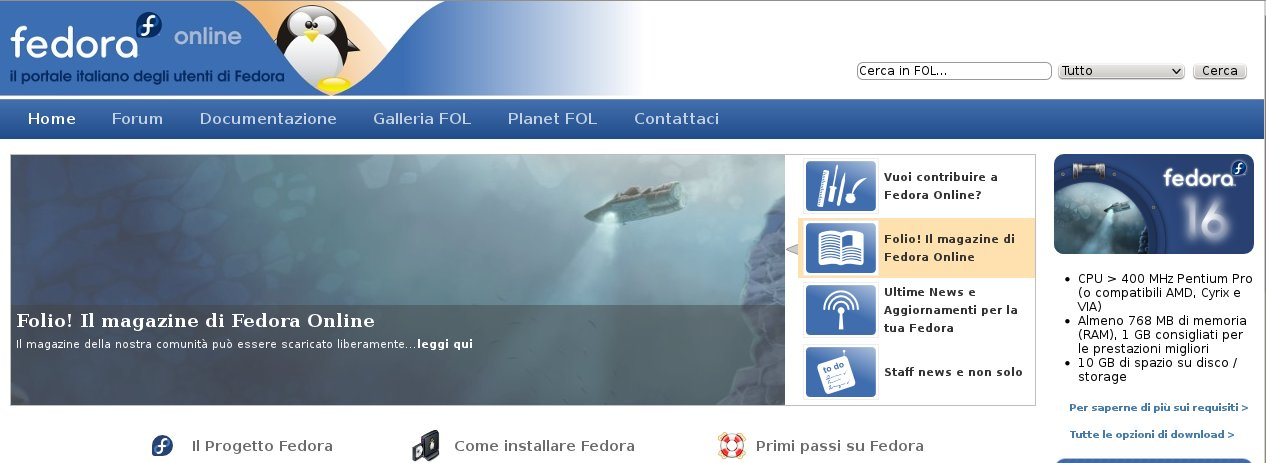
\includegraphics[scale=.20]{articoli/editoriale/immagini/fol.jpeg}
\caption{il nuovo portale FedoraOnLine\label{fig 1:Il nuovo portale FedoraOnLine}}
\end{figure}

Verranno anche portate avanti e sviluppate tematiche connesse a Fedora, al Fedora Project ed a quant'altro ruoti intorno ai sistemi GNU/Linux con l'intenzione di accorciare la distanza che intercorre tra gli utenti ed il Fedora Project, scrivendo diffusamente sulle qualità e, perchè no?, dei difetti della struttura organizzativa, conoscendo anche da vicino chi è impegnato nelle varie attività ad esso correlate.\\

Ma non solo! FedoraOnLine, tramite questa rivista, vuole cercare di ridurre quelle difficoltà che i nuovi utenti riscontrano nell'avvicinamento a GNU/linux, createsi sia per oggettive complessità tecniche sia per stereotipi che non hanno senso di esistere; in sostanza proveremo a descrivere una visione a 360 gradi dell'open source e del free software.\\

Non abbiamo mire editoriali, non siamo professionisti della carta stampata, nè vogliamo esserlo, ma questa iniziativa è rivolta a coloro, soprattutto, che hanno voglia di guardare e capire cosa ci lega ad uno sviluppatore dell'Illinois, ad un grafico dell'India e a chissà quante altre persone.\\

Basta un gesto del mouse o premere un carattere sulla tastiera affinchè i {\itshape linuxiani} si pongano delle domande.\\

Già qualche anno fa eravamo riusciti a trasformare una idea in qualcosa di buono e di utile, scrivendo un libro sulla release 9 di Fedora, che fornisse un supporto per l'avvicinamento al nostro sistema operativo.\\

\begin{figure}[htbp]
\centering
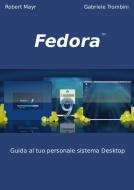
\includegraphics[scale=.55]{articoli/editoriale/immagini/libro_copertina.jpg}
\caption{Fedora 9, il libro\label{fig 2:Fedora 9, il libro}}
\end{figure}

Ovviamente siamo del tutto aperti a consigli, critiche e a correzioni da parte di chi legge ed il riferimento a cui inviare tutto ciò che vi dovesse venire in mente è {\itshape redazione@fedoraonline.it}.\\

In questo primo numero cominceremo ad introdurre il Fedora Project, descrivendone gli obiettivi e parlandone un po' con chi ne è addentro, parleremo dei motivi e dei retroscena che ci hanno portato al restyling del nostro sito, vedremo come avvicinarci alla shell Linux, approfondiremo software, illustreremo i servizi di Fedora, daremo una prima occhiata al kernel e comincieremo a studiare il sistema di packaging di Fedora, cioè gli rpm.\\

Ovviamente non potremo fare a meno di gettare uno sguardo sul futuro prossimo di Fedora, alle features annunciate per la release numero 17 la cui uscita è prevista a Maggio 2012, come da roadmap che si può trovare alla pagina {\itshape http://fedoraproject.org/wiki/Schedule}.\\

Niente altro da aggiungere, al momento, specificando, però, che l'impostazione grafica della rivista sarà soggetta a miglioramenti e che per il momento la cadenza per la pubblicazione dei numeri successivi a questo è ancora lontana dall'essere definita.\\

Il successo di questa iniziativa dipende dai nostri lettori, vi aspettiamo. 




\clearpage
\twocolumn[
\begin{center}
\title{\color[cmyk]{1, 0.57, 0, 0.38}{\Huge\bfseries Fedora Project\\}} % definisco il titolo dell'articolo
\author{\scriptsize Gabriele Trombini (mailga@fedoraonline.it)} % definisco l'autore e altre informazioni
\date{}
\end{center}
{\color[cmyk]{1, 0.46, 0, 0}\LARGE Il Fedora Project - comprensione di un grande fenomeno legato al software libero}\\
\maketitle
\normalsize
\doublespacing
\hfill
]
\lettrine[lines=1, loversize=0.1, lraise=0.1]{\color[cmyk]{0.5, 0, 1, 0}\bfseries C}{}redo che tutti noi ci siamo chiesti almeno una volta quale lavoro stava dietro al nostro sistema operativo. Quali fossero i mezzi utilizzati e quante persone erano impegnate nel suo sviluppo.\\

Tutto è riconducibile al Fedora Project {\itshape (http://fedoraproject.org/)} che si può definire un contenitore per le idee che vengono portate avanti da singoli utenti che condividono il proprio lavoro.\\

\begin{figure}[htbp]
\centering
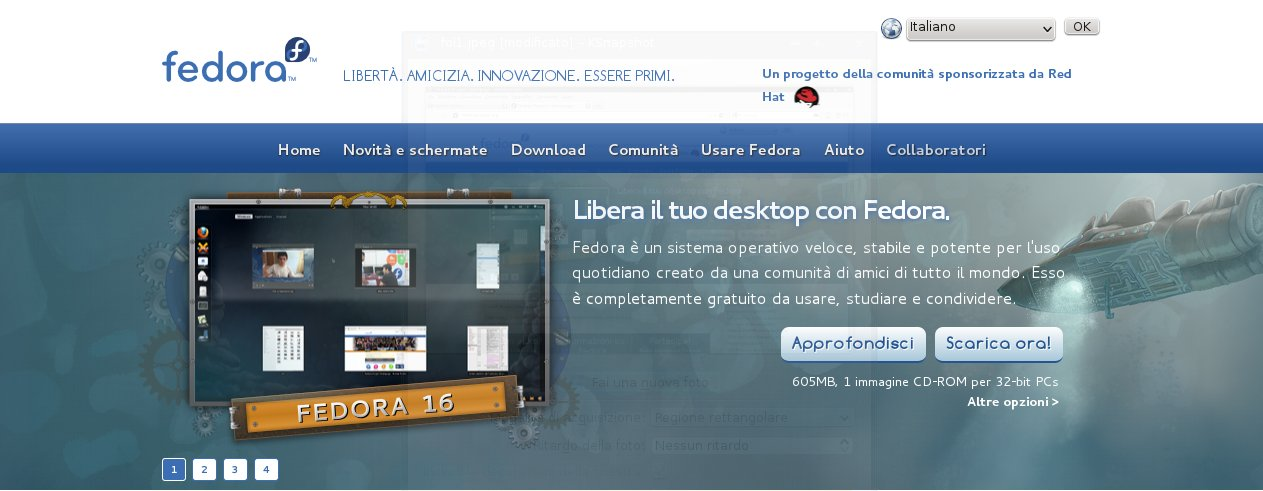
\includegraphics[scale=.20]{articoli/varie/immagini/fp.jpeg}
\caption{Il sito del Fedora Project\label{Fig.1: Fedora Project}}
\end{figure}

Chiunque voglia impegnarsi attivamente nel progetto potrebbe trovare un po' difficoltoso avventurarsi all'interno del suo sito web in quanto la sua organizzazione è molto capillare.\\

Vediamo, in questo articolo, di chiarire un po' le idee degli utenti.\\

Innanzi tutto è bene precisare i termini del legame tra Red Hat ed il Fedora Project, come spiegato all'indirizzo web {\itshape http://it.redhat.com/resourcelibrary/arti cles/relationship-between-fedora-and-\\ rhel}, dove ben si definisce che sono due entità separate, la prima con l'obiettivo dell'IT, la seconda a vantaggio della comunità:\\
{\itshape ``Le dimensioni e l'esperienza della comunità di Fedora, rendono Fedora l'incubatrice e il terreno di prova ideale per le funzioni che, in seguito, verranno integrate in Red Hat Enterprise Linux. Per soddisfare i requisiti di qualità e affidabilità che rendono Red Hat Enterprise Linux la scelta ideale per le applicazioni di importanza cruciale, i test e processi di controllo di qualità di Red Hat Enterprise Linux sono separati e distinti da quelli di Fedora.\\

Fedora: sviluppo rapido della tecnologia più recente.\\

La comunità di Fedora è composta da migliaia di utenti, collaboratori e sostenitori, i quali interagiscono tramite i forum online, le mailing list ed i wiki per sostenersi l'un l'altro. Con uno sviluppo e un ciclo di distribuzione molto rapidi, Fedora fornisce la tecnologia più recente sulle piattaforme hardware attuali.\\

Red Hat Enterprise Linux: piattaforma open source stabile e supportata.\\

Se si sceglie di eseguire Red Hat Enterprise Linux, si entra in stretto contatto con il principale fornitore di soluzioni open source. Non solo si ottiene una piattaforma affidabile e stabile, con un ciclo di vita di 10 anni, ma si può godere anche dei vantaggi offerti da organizzazioni internazionali di progettazione, consulenza e assistenza. Una sottoscrizione Red Hat Enterprise garantisce l'accesso a software e manutenzione di alta qualità, oltre alle informazioni e all'assistenza che si estendono al ciclo di vita e all'architettura dell'intera infrastruttura.''} \\

Nella pagina del sito Fedora {\itshape http://fedo raproject.org/sponsors} si specifica che la casa madre mette a disposizione del progetto infrastrutture, personale e finanziamenti:\\
{\itshape ``Red Hat, Inc. è lo sponsor principale per il Fedora Project. Red Hat fornisce al Fedora project una varietà di risorse, che includono il supporto dei dipendenti a tempo pieno, infrastrutture hardware e di banda, finanziamento degli eventi e consulenza legale.''}\\

Ricordiamoci bene, però, che Red Hat non è Fedora.\\

Il Fedora Project è il contenitore ideale dove, chiunque di noi, può sostenere, integrare,
migliorare, creare i progetti che diventeranno parte integrante dell'idea che
sta alla base di tutto questo.\\


Non è possibile scindere la totalità del progetto dal sistema operativo perchè
esso è l'emanazione ultima di quello che è stato creato; la sua punta di
diamante.\\

Prima di essere un sistema operativo, Fedora è un crocevia di libero pensiero.
E' riduttivo, infatti, qualificare il Fedora Project come un sistema operativo;
alle spalle di esso c'è una comunità internazionale che sostiene i settori di
sviluppo.\\

Le attività del progetto son molteplici, dallo sviluppo di applicazioni, allo
sviluppo di rami del kernel, da quello del design a quello della
internazionalizzazione, da quello del marketing a quello del web e altro ancora.\\

La distanza tra l'utilizzatore ed il progetto, non è poi così lontana, anzi, è a
portata di mano! Una semplice digitazione di {\itshape www.fedoraproject.org} sulla barra degli
indirizzi e si è già dentro, immersi nelle possibilità che ti può
dare.\\
I valori alla base del lavoro di tutte le persone coinvolte, sono quattro:
\begin{itemize}
\item 
\includegraphics[scale=.20]{articoli/varie/immagini/4f-freedom.png} libertà 
\item 
\includegraphics[scale=.20]{articoli/varie/immagini/4f-friends.png} comunità
\item 
\includegraphics[scale=.20]{articoli/varie/immagini/4f-features.png} condivisione
\item 
\includegraphics[scale=.20]{articoli/varie/immagini/4f-first.png} innovazione
\end{itemize}
e ciascun contributo deve rispettare questi valori.\\

In questo articolo vorrei soffermarmi sul concetto di comunità, estesa al mondo intero, entro la quale ciascuno di noi può (come detto) dare il proprio contributo.\\

I mezzi a disposizione degli utenti sono davvero molti e molto potenti, a cominciare proprio da una area di interesse ben definita.\\

Dividiamo pure in macroaree all'interno delle quali è possibile trovare il proprio spazio specifico e ben dettagliato:
\begin{itemize}
\item 
\includegraphics[scale=.20]{articoli/varie/immagini/join-writer.png} redattore 
\item 
\includegraphics[scale=.20]{articoli/varie/immagini/join-designer.png} disegnatore
\item 
\includegraphics[scale=.20]{articoli/varie/immagini/join-people.png} comunicatore
\item 
\includegraphics[scale=.20]{articoli/varie/immagini/join-osdevel.png} sviluppatore del sistema operativo
\item 
\includegraphics[scale=.20]{articoli/varie/immagini/join-translator.png} traduttore
\item 
\includegraphics[scale=.20]{articoli/varie/immagini/join-webdevel.png} sviluppatore web o amministratore
\end{itemize}
Prima di andare ad analizzare questi ruoli, è bene specificare il ruolo del FAS (Fedora Account System), a cui ci si deve iscrivere, per poter iniziare la propria attività in favore di Fedora.\\

Il FAS, raggiungibile all'indirizzo {\itshape https:// admin.fedoraproject.org/accounts/user/ new} è il sistema per poter richiedere l'associazione ad un gruppo, gestito dagli amministratori. Infatti gli iscritti sono tutti gli appartenenti ai gruppi di lavoro ed è all'interno di esso che è possibile sottoscrivere la domanda di ammissione.\\

Avere un account FAS valido ci permette di avere uno spazio personale nel wiki all'interno del quale è possibile descrivere le proprie esperienze ed i propri contributi. \\
\begin{figure}[htbp]
\centering
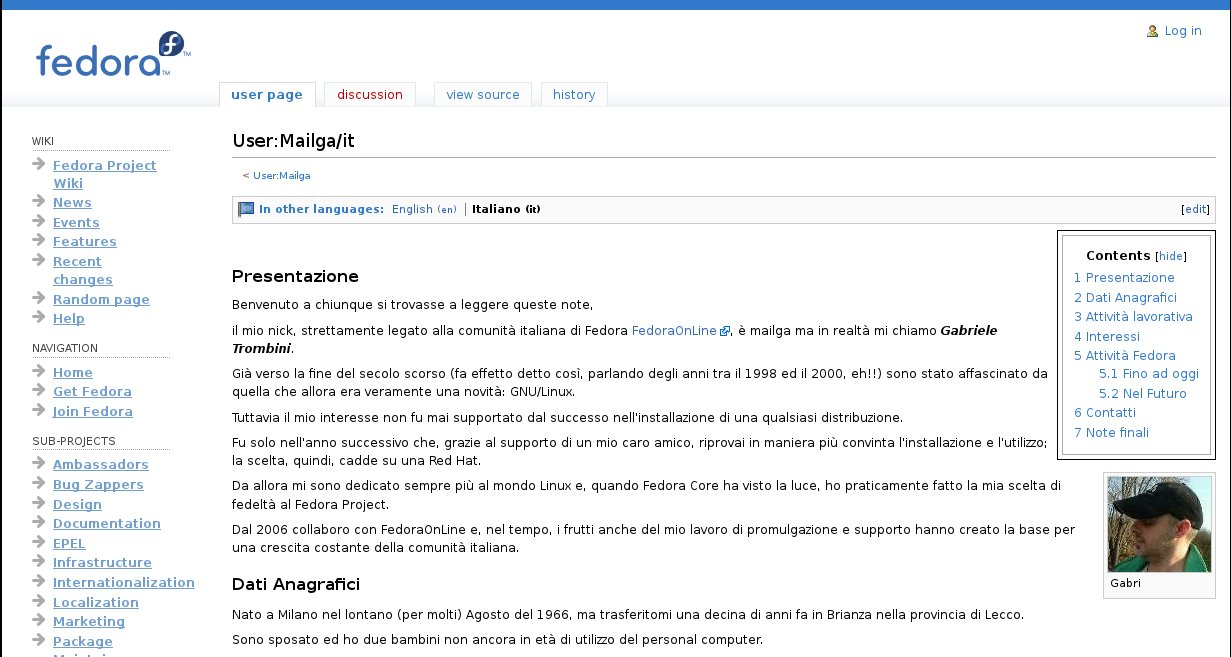
\includegraphics[scale=.20]{articoli/varie/immagini/mailga-wiki.jpeg}
\caption{pagina wiki Mailga\label{Fig.1: server git}}
\end{figure}

Nella pagina web {\itshape https://fedoraproject. org/wiki/Projects} è possibile avere una lista dettagliata e le spiegazioni dei vari progetti.\\

\begin{figure}[!h]
\centering
{\bfseries Redattore 
\includegraphics[scale=.30]{articoli/varie/immagini/join-writer.png}}
\end{figure}
Il ruolo di redattore è particolarmente adatto a coloro che hanno particolare facilità di scrittura. In questa area trovano spazio sia i collaboratori che scrivono i contributi, sia coloro che li traducono nelle varie lingue.\\

\begin{figure}[!hp]
\centering
{\bfseries Disegnatore 
\includegraphics[scale=.30]{articoli/varie/immagini/join-designer.png}}
\end{figure}
In questo gruppo potrà trovare una attività congeniale chi è particolarmente abile nelle arti grafiche.\\

\begin{figure}[!h]
\centering
{\bfseries Comunicatore 
\includegraphics[scale=.30]{articoli/varie/immagini/join-people.png}}
\end{figure}
Questa macrosezione è pensata per le persone che hanno attitudini alla comunicazione, sia essa in pubblico che attraverso attività di marketing.\\

\begin{figure}[!h]
\centering
{\bfseries Sviluppatore sistema operativo 
\includegraphics[scale=.30]{articoli/varie/immagini/join-osdevel.png}}
\end{figure}
I gruppi appartenenti a questa categoria sono fondamentali per la riuscita del sistema operativo. Le persone con conoscenze sulla programmazione potrebbero partecipare alle attività degli sviluppatori.\\

\begin{figure}[!h]
\centering
{\bfseries Traduttore 
\includegraphics[scale=.30]{articoli/varie/immagini/join-translator.png}}
\end{figure}
Un'altra sezione veramente importante per la diffusione del sistema nei vari paesi del mondo è proprio questa. Chiunque possa aiutare nella traduzione di tutta la documentazione Fedora nella propria lingua madre, avendo conoscenze dell'inglese, troverà ampio spazio.\\

\begin{figure}[!h]
\centering
{\bfseries Sviluppatore web/sysadmin 
\includegraphics[scale=.30]{articoli/varie/immagini/join-webdevel.png}}
\end{figure}
Infine, chi è addentro al linguaggio web, allo sviluppo di applicazioni web e/o all'amministrazione dei sistemi Linux può davvero risultare fondamentale per l'infrastruttura del Fedora Project.\\

Tutto quanto gira intorno e all'interno del progetto è nato nello spirito open e free, che abbiamo visto essere tra i fondamenti delle attività ad esso legate.\\

Ed è proprio in questo che si deve partire per comprendere il fenomeno, perchè chi non intende lasciare libera una comunità di proporre, di decidere e anche di sbagliare, non potrà sperare di ottenere risultati apprezzabili.\\

\clearpage
\twocolumn[
\begin{center}
\title{\color[cmyk]{1, 0.57, 0, 0.38}{\Huge\bfseries Intervista a: Gianluca Sforna\\}} % definisco il titolo dell'articolo
\author{\scriptsize Gabriele Trombini (mailga@fedoraonline.it)} % definisco l'autore e altre informazioni
\date{}
\maketitle
\normalsize
\hfill
\end{center}
{\color[cmyk]{1, 0.46, 0, 0}\LARGE Le interviste di Folio - incontriamo Gianluca Sforna}  \\
\small\sl Abbiamo chiesto al nostro amico Gianluca di rispondere a 10 domande, sperando anche di metterlo in difficoltà. La qualità delle risposte non ci ha affatto sorpreso.\\
]
\begin{figure}[htbp]
\centering
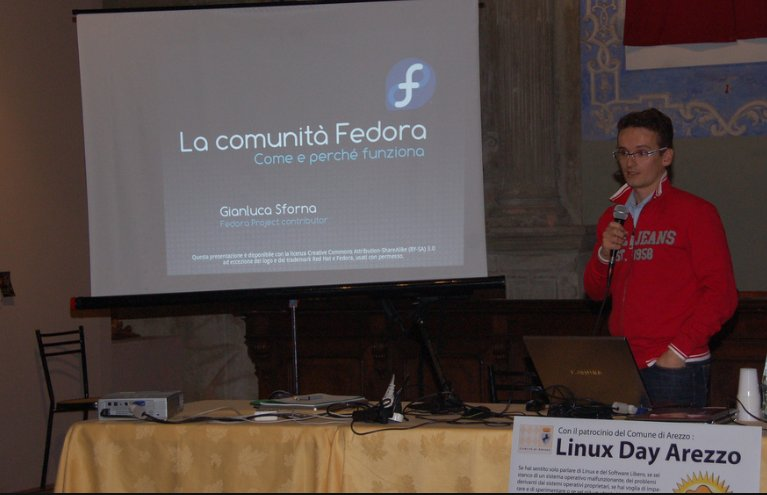
\includegraphics[scale=.35]{articoli/varie/immagini/giallu.jpg}\\
\end{figure}
\singlespacing
\definecolor{shadecolor}{cmyk}{0, 0, 0, 0.1}
\begin{shaded}
{\footnotesize
\color[cmyk]{1, 0.57, 0, 0.38}
\emph{Chi è \textbf{Gianluca Sforna? (@giallu)}\\
classe 1972, programmatore e sysadmin.\\
Inizia a lavorare stabilmente su Linux nel 1999 con Red Hat Linux 6.0;
nel 2003 diventa prima utente e poi contributor del progetto Fedora.\\
Oggi è maintainer di diversi pacchetti RPM ospitati tra repository
ufficiali (Fedora, RPMFusion) e privati, traduttore ed ambassador del
progetto.\\ Il suo blog: \\http://morefedora.blogspot.com}
}
\end{shaded}
\bigskip
\onehalfspacing
\emph{\textbf{FOL: 1) chi è il Fedora Project?}}\\
\emph{\textbf{Giallu: }}Il progetto non è nessuno in particolare, ma in effetti si può dire che tutti i partecipanti al progetto in qualche modo sono Fedora: infatti anche il più piccolo dei contributi permette al progetto e agli altri partecipanti di crescere e migliorarsi, quindi il progetto nel suo complesso si può sicuramente considerare ``figlio'' di ogni contributor. Non a caso ho partecipato ad EuroPython 2011 con questo badge:
\begin{figure}[htbp]
\centering
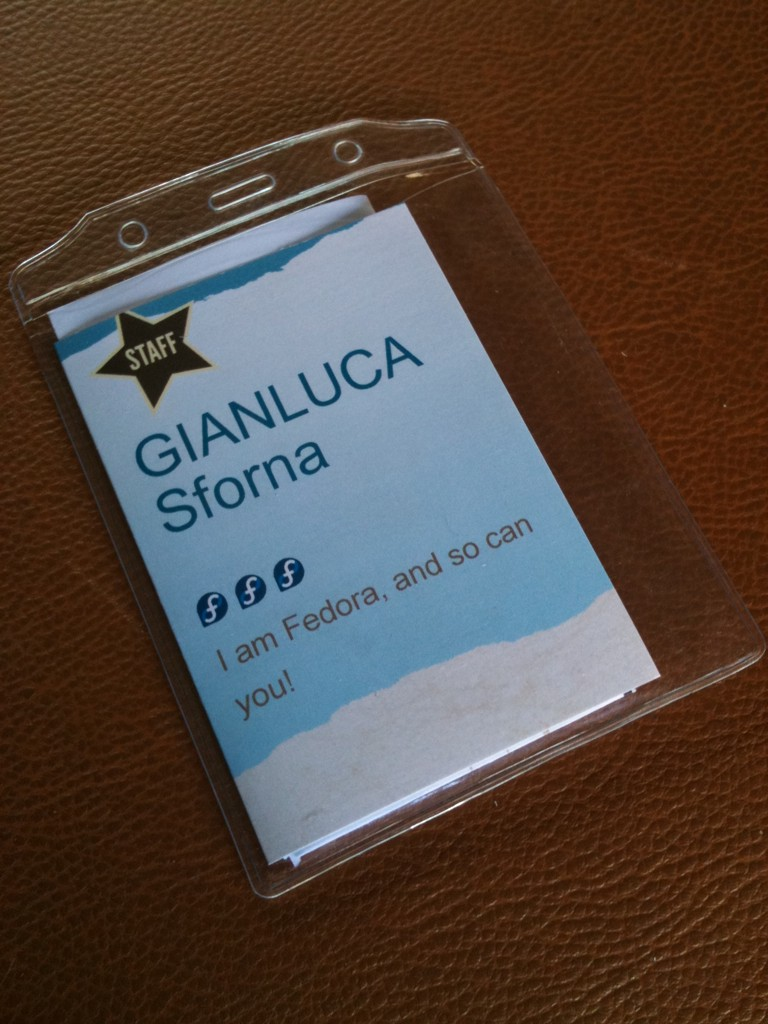
\includegraphics[scale=.10]{articoli/varie/immagini/badge.jpg}\\
\end{figure} \\

\emph{\textbf{FOL: 2) gli ambassador promuovono il progetto o il sistema operativo?}}\\
\emph{\textbf{Giallu: }}Direi entrambi: gli Ambassador promuovono senz'altro il progetto e i suoi valori, ma è chiaro che la distribuzione era e rimane il prodotto principale e più visibile quindi trovo difficile che si possa scindere i due aspetti.\\

\emph{\textbf{FOL: 3) sbaglia qualcosa, il Fedora Project? Se sbaglia, in che modo?}}\\
\emph{\textbf{Giallu: }}Un progetto così grande sicuramente ha sia punti di forza che debolezze. E' però praticamente impossibile dare un giudizio assoluto, visto che tutto dipende da cosa si usa come metro per definirne il successo. Se per dire mi aspetto dal progetto una distribuzione che posso installare su un server  e supportare per una decina di anni, troverò che si stanno compiendo molti errori. Lo stesso se mi aspetto una distribuzione ``rolling'', che includa sempre e comunque solo le ultime versioni di ogni software. 
Da notare che gli obiettivi del progetto non sono ``statici'' ma sono stati più volte sviluppati, raffinati e chiariti; ad oggi, se esaminiamo la pagina del wiki che li elenca (https://fedoraproject.org/\\wiki/Objectives) direi che il progetto nel suo complesso è decisamente sulla buona strada.\\

\emph{\textbf{FOL: 4) cosa rubereste a Debian, a Slackware ed a gentoo?}}\\
\emph{\textbf{Giallu: }}Premesso che dopo tanti anni di uso esclusivo di Fedora (e derivate) non conosco bene la situazione dei nostri ``cugini'', devo dire che di Debian ammiro l'organizzazione complessiva che riesce a "tenere" un gran numero di utenti e sviluppatori anche a dispetto dei loro ingombranti vicini di casa.\\

\emph{\textbf{FOL: 5) non vi pare che i linux day e i Fudcon siano eventi riservati ad una ristretta utenza, in fondo si riferiscono sempre agli stessi ambienti?}}\\
\emph{\textbf{Giallu: }}Credo che i due eventi siano profondamente diversi: se i Linux Day si rivolgono ad una ampia platea essendo un evento divulgativo per definizione (anche se poi sono tanti i partecipanti già introdotti alla filosofia del software libero), il FUDCon mi sembra più un evento del "fare" e per questo sicuramente ricco di utenti avanzati e sviluppatori che approfittano della occasione di aggregazione per accelerare quelle attività di sviluppo a volte rallentate dalla distanza fisica tra i contributor. Concordo comunque sul fatto che siano eventi di ``nicchia'', visto che comunque ancora oggi, a dispetto di tutti i progressi fatti, Linux continua ad essere il settore ``Altro'' vicino a ``Windows'' e ``MacOSX'' dei diagrammi a torta.\\

\emph{\textbf{FOL: 6) dove pensate che si possa essere più incisivi nella promozione?}}\\
\emph{\textbf{Giallu: }}Direi un po' ovunque: scuole, università, LUG, eventi, aziende pubbliche private etc. 
Ad oggi mi pare evidente che altre distribuzioni siano riuscite ad attrarre un grosso numero di utenti (che è comunque un bene visto che per lo più provengono da altri sistemi operativi). Se consideriamo che Fedora si rivolge ad un pubblico più consapevole la situazione non è drammatica, ma siccome penso sia più difficile ``convertire'' un utente piuttosto che acquisirlo la prima volta, spero che lo sforzo di marketing sul progetto sia sempre più efficace.\\

\emph{\textbf{FOL: 7) perchè l'utente dovrebbe usare fedora e non altre distro? solo per il free software, non vi pare un po' troppo idealistico?}}\\
\emph{\textbf{Giallu: }}Il software libero l'utente lo trova in tutte le distro; non tutte però ti garantiscono che la totalità dei contenuti siano effettivamente ridistribuibili; per dire, se sei una azienda ed hai intenzione di produrre e vendere un prodotto hardware o software basato su Linux, Fedora può essere una ottima scelta proprio per questo motivo. La altre motivazioni si trovano nella metodologia di sviluppo: collaborazione con gli upstream (i progetti su cui si basa la distribuzione tipo kernel, GNOME, KDE, etc), aggiornamenti rapidi (siamo quasi sempre i primi a fornire le ultime versioni disponibili), totalità degli strumenti usati disponibili (per cui chiunque può farsi la ``sua'' distribuzione derivata)
L'utente comune tende invece a dare valore ad altre caratteristiche, ad esempio che i suoi mp3 o DVD si possano riprodurre semplicemente cliccandoci sopra (per inciso, questa cosa funziona proprio in questo modo in Fedora, previa attivazione dei repository RPMFusion) oppure che la esistenza di driver proprietari venga notificata automatizzandone l'installazione.
Purtroppo questo a volte si scontra con il fatto che Fedora punta alla produzione e integrazione del migliore e più recente software libero: per esempio, molto spesso nel passato i driver ATI disponibili erano incompatibili con il server X o con il kernel distribuiti in quel momento da Fedora, e solo con mesi di ritardo AMD ha provveduto a fornire driver funzionanti; in queste condizioni non c'è molto che il progetto possa fare, se non lavorare ancora di più per rendere inutili tali driver, sostituiti dalle loro controparti open.\\

\emph{\textbf{FOL: 8) ritieni di aver fatto tutto il possibile per promuovere Fedora?}}\\
\emph{\textbf{Giallu: }}Sicuramente no:  il lavoro non manca mai, ma il tempo e l'energia a volte non sono facili da trovare. Per questo penso sia sempre prioritario trovare e motivare nuovi contributor, così che la riserva di idee e manodopera per nuove iniziative sia sempre alimentata.\\

\emph{\textbf{FOL: 9) Fedora avrà un ritorno dall'utenza italiana?}}\\
\emph{\textbf{Giallu: }}Sicuramente. La barriera alla partecipazione al progetto è sempre più bassa e chiunque, a prescindere dalle proprie capacità tecniche, può dare un contributo. Basta guardarsi un po' intorno per scoprire il team più adatto alle proprie inclinazioni e capacità ed iniziare!\\

\emph{\textbf{FOL: 10) Come siamo noi italiani rispetto alla totalità del progetto?}}\\
\emph{\textbf{Giallu: }}Ci sono team ben più organizzati, ma devo dire che gli Italiani nel progetto non mancano a tutti i livelli. Se solo trovassimo il modo di aumentarne la coesione credo che saremmo tra i gruppi più importanti del progetto...
\\

\clearpage
\twocolumn[
\begin{center}
\title{\color[cmyk]{1, 0.57, 0, 0.38}{\Huge\bfseries Fedora Inside\\}} % definisco il titolo dell'articolo
\author{\scriptsize Gabriele Trombini (mailga@fedoraonline.it)} % definisco l'autore e altre informazioni
\date{}
\end{center}
{\color[cmyk]{1, 0.46, 0, 0}\LARGE Una collaborazione speciale - Andrea Veri}\\
\maketitle
\normalsize
\doublespacing
\hfill
]
\onehalfspacing
\lettrine[lines=1, loversize=0.1, lraise=0.1]{\color[cmyk]{0.5, 0, 1, 0}\bfseries F}{}in da questa prima uscita e con grande piacere, possiamo avvalerci della collaborazione di un amico che opera nell'infrastruttura del Fedora Project e in posizioni prestigiose all'interno del panorama GNU/Linux.\\ 

Visto la natura delle argomentazioni che Andrea tratterà all'interno di Folio (principalmente sicurezza e sistemi, talvolta spiegherà dinamiche viste dall'interno del progetto) la presenza dei suoi contributi, ovviamente, non potrà avere il carattere della continuità.\\

Andrea Veri è un ventiduenne studente della facoltà di Giurisprudenza dell'Università di Udine.\\

Da sempre appassionato di informatica, iniziò nel 2006 a contribuire nei campi della documentazione e del packaging di applicazioni in Ubuntu per poi spostarsi successivamente in Debian, dove ottenne il titolo di sviluppatore ufficiale con i relativi accessi all'archivio principale della distribuzione.\\

Dal 2009, iniziò la sua collaborazione con il progetto GNOME nel quale ricopre alcune posizioni di carattere infrastrutturale, nello specifico, si occupa di amministrare e gestire il server LDAP di GNOME e presiede la GNOME Membership \& Elections Committee, la quale si occupa di valutare, accettare o rifiutare le richieste di appartenenza alla Fondazione GNOME e non solo: tale commissione è, inoltre, incaricata di organizzare le elezioni della Board of Directors a Giugno prima del GUADEC.\\

Dal 2010, Andrea si sposta, pur mantenendo attive le altre sue collaborazioni con Debian e GNOME, in Fedora.\\

I primi gruppi di lavoro furono relativi alle traduzioni in lingua italiana, al gruppo Insight ed a quello Infrastructure.\\

Seguì poi la creazione del sub-planet JustFedora e la successiva candidatura alla Board di Fedora.\\

Al momento, le sue attività si concentrano maggiormente nel packaging RPM e nella amministrazione di sistema di alcune macchine utilizzate dall'infrastruttura di Fedora.\\
\clearpage
\twocolumn[
\begin{center}
\title{\color[cmyk]{1, 0.57, 0, 0.38}{\Huge\bfseries Il nuovo FedoraOnLine: motivazioni e curiosità\\}} % definisco il titolo dell'articolo
\author{\scriptsize Gabriele Trombini (mailga@fedoraonline.it)} % definisco l'autore e altre informazioni
\date{}
\end{center}
{\color[cmyk]{1, 0.46, 0, 0}\LARGE FOL 2 - il percorso pieno di imprevisti}\\
\maketitle
\normalsize
\doublespacing
\hfill
]
\onehalfspacing
\lettrine[lines=1, loversize=0.1, lraise=0.1]{\color[cmyk]{0.5, 0, 1, 0}\bfseries I}{}l nostro webmaster, come molti di voi certamente sapranno, è uno stakanovista del lavoro in FedoraOnLine, un vulcano di idee, ed è sempre pronto a valutare qualsiasi possibilità di crescita.\\

Da molto tempo, all'interno dello staff, si discuteva circa un possibile rinnovamento grafico e concettuale del sito. Le idee erano molte ma la focalizzazione degli strumenti atti a raggiungere lo scopo erano ben remoti dall'essere stabiliti.\\

La questione non si poneva solo in termini di layout, la rivisitazione avrebbe dovuto riguardare la totalità del sito: si trattava di scegliere il cms in sostituzione di Xoops, che ci avrebbe permesso di gestire in maniera più efficace le sezioni presenti.\\

Prese così forma l'obiettivo da raggiungere, che comprendeva sia il cms che dei gestori di contenuti (in primis il forum stesso e la sezione documentazione).\\

Il lavoro che si presentava era decisamente superiore alle forze presenti nello staff, anche perchè il forum ``vecchia versione'' doveva avere continuità.\\

Pertanto, definite le zone di interesse e gli strumenti per la loro gestione (Drupal a livello di cms, fluxbb a livello di forum e mediawiki per la parte documentale), abbiamo cominciato a lavorare sulle varie sezioni, ricercando anche dei validi collaboratori per ottenere i risultati sotto gli occhi di tutti.\\

Virus, Trpost ed io avremmo continuato a gestire il forum insieme, mentre Robyduck, MarioS e Pagnolo avrebbero cominciato a vedere come mettere insieme tutti gli strumenti che erano stati scelti.\\

Era l'estate dell'anno scorso e Virus ci mise a disposizione un server git per poter mettere insieme il lavoro fatto in comune.\\

\begin{figure}[htbp]
\centering
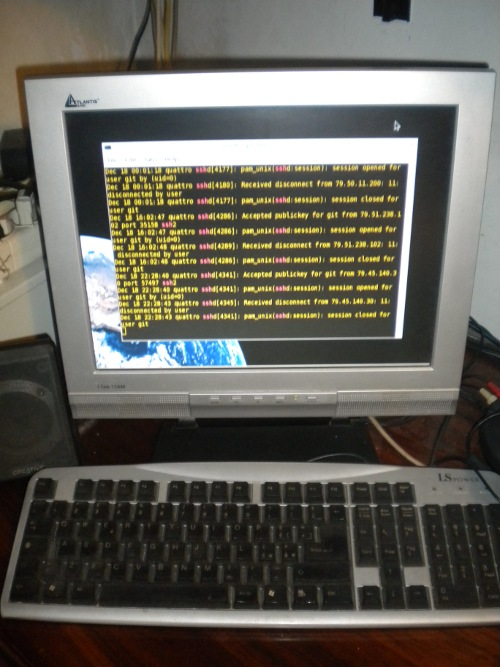
\includegraphics[scale=.10]{articoli/editoriale/immagini/server_git.jpg}
\caption{Il nostro server git\label{Fig.1: server git}}
\end{figure}

Il primo grosso problema che si presentò era il trasferimento del database di Fol versione 1.0 in quello che sarebbe divenuto Fol 2.0, perchè non aveva senso perdere la nostra storia.\\

Il secondo grosso problema, che ci era sembrato insormontabile, inizialmente, era dato dal login unificato tra Drupal e Fluxbb (non aveva senso mantenerlo anche per Mediawiki, visto che solo i redattori iscritti in mailing list, possono fornire contributi).\\

In entrambi i casi il lavoro fu abbastanza duro e richiedemmo aiuto anche ai nostri cugini d'oltralpe di fedora-fr.org, i quali ci indirizzarono verso una soluzione con delle criticità troppo onerose per le nostre energie.\\

Nel frattempo Robyduck e Pagnolo si occupavano della sistemazione grafica, uniformandola nei diversi programmi coadiuvati dai collaboratori per la parte grafica, lo storico Tuzzer ed Ilnanny mentre il nostro MarioS ricercava un modo più semplice per poter fare il login unificato e per il trasferimento dei dati da un database all'altro.\\

Tutto procedeva, a Folio era stata data una priorità ovviamente secondaria, senonchè, a causa di scelte personali Trpost si distaccò dal nostro gruppo di lavoro e impegni lavorativi portavano lontano dal progetto anche Tuzzer.\\

Se contiamo il fatto che alcuni utenti, solitamente presenti e attivi in seno alle notizie ed al forum, che ci avevano dato disponibilità a prendere in mano un settore di interesse, a causa di problemi personali non hanno potuto anch'essi proseguire nella collaborazione, ci siamo trovati, ad un certo punto, in grossa difficoltà.\\

Riassumendo, eravamo bloccati sulla soluzione del login (il trasferimenti da un database all'altro non era più un problema), la gestione del forum aveva subito una defezione, il supporto grafico era dimezzato e alcuni collaboratori non potevano darci una mano.\\

Per di più bisognava cominciare a tracciare le linee per la redazione di Folio.\\

Il tutto faceva prendere una brutta piega al lavoro, che subiva, quindi, un rallentamento.\\

La svolta ci fu quando MarioS ha trovato il modo per il login unico (ricordiamo l'importanza di avere un login nella home del sito e non doverlo ripetere qualora si entri nel forum) e con il mio spostamento sull'attività di Mediawiki (insieme a Robyduck, che si occupava di tutto, e di Zamingas).\\

Mediawiki aveva bisogno di essere impostato per quanto riguarda le due pagine di fondamentale importanza, ``contribuisci'' e ``convenzioni di scrittura'', che furono fatte in breve tempo da me e da Robyduck, dopo aver stabilito che anzichè appoggiarci al server git, per la parte documentale sarebbe stato meglio creare online la sezione.\\

Passammo poi, con il contributo di ilnanny, MarioS stesso e Zamingas, a importare le guide dal vecchio sito al nuovo; operazione tediosa ma relativamente breve.\\

Facendo le somme, a quel punto capimmo che era cominciata la fase di discesa; Drupal era ad un passo dalle rifiniture finali, il forum era stato importato nel nuovo database di Fluxbb, Mediawiki era finito e lo script di login era praticamente terminato.\\

Ormai ce l'avevamo fatta, per cui mi sono buttato a capofitto su Folio, se non che, la mia decisione iniziale di redigerlo con Scribus faceva a pugni con quello che nel web viene solitamente fatto: cioè l'utilizzo di Latex.\\

Dovevo cominciare daccapo, leggere e studiare, studiare e capire un linguaggio non propriamente facile anche se redditizio in termini di resa.\\

A questo punto, ed è storia di oggi, siamo online, con dei ritorni positivi e con l'uscita di questo numero di Folio.\\

\begin{figure}[htbp]
\centering
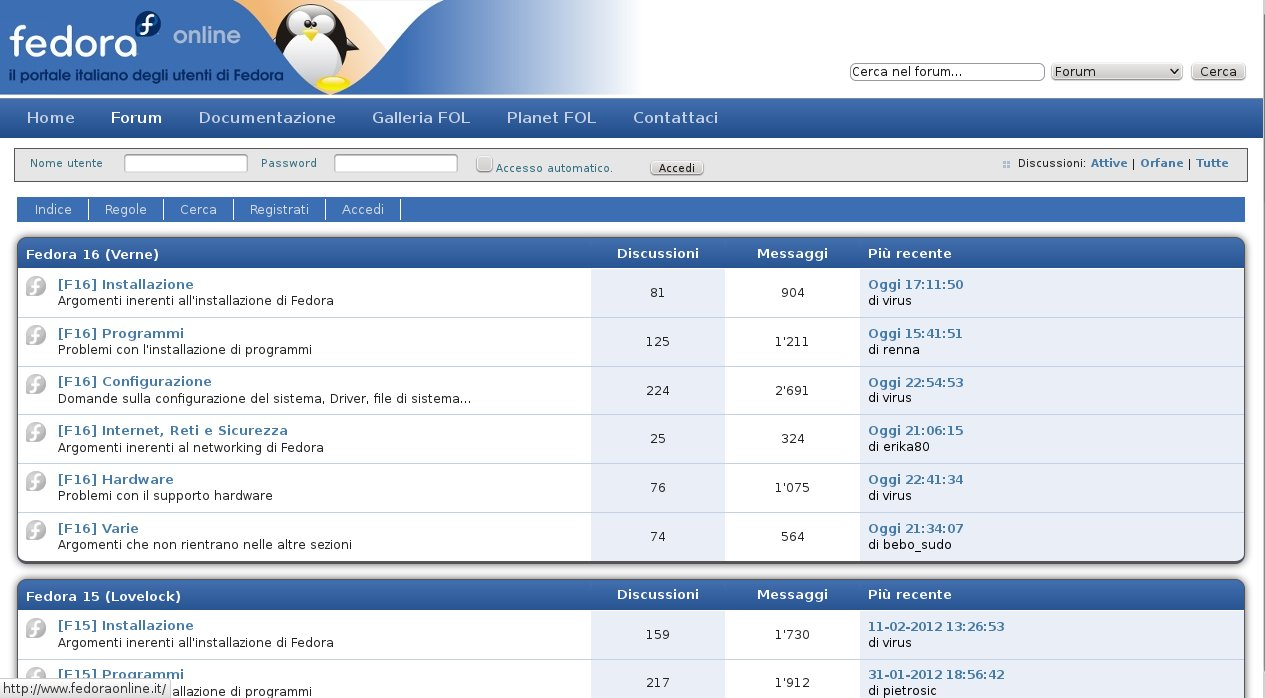
\includegraphics[scale=.20]{articoli/editoriale/immagini/forum_fol.jpeg}
\caption{Il nostro forum\label{Fig.1: forum}}
\end{figure}

La missione è compiuta, siamo orgogliosi di aver messo a disposizione delgli utenti uno strumento che possa dare risposta alle richieste.\\

E Virus?
Ragazzi! Senza Virus che ha retto sulle proprie spalle il carico del forum senza creare disagio agli utenti, non ho difficoltà ad ammettere che probabilmente tutto questo non avrebbe potuto essere così.\\

That's all, folks!


\clearpage
\twocolumn[
\begin{center}
\title{\color[cmyk]{1, 0.57, 0, 0.38}{\Huge\bfseries Linea di comando\\}} % definisco il titolo dell'articolo
\author{\scriptsize Gabriele Trombini(mailga@fedoraonline.it)} % definisco l'autore e altre informazioni
\date{}
\end{center}
{\color[cmyk]{1, 0.46, 0, 0}\LARGE (Parte prima) Consolle virtuale e terminale - la base dei sistemi GNU/Linux}\\
\maketitle
\normalsize
\doublespacing
\hfill
]
\definecolor{shadecolor}{cmyk}{0, 0, 0, 0.8}
\onehalfspacing
\lettrine[lines=1, loversize=0.1, lraise=0.1]{\color[cmyk]{0.5, 0, 1, 0}\bfseries L}{}a linea di comando è sicuramente un ostacolo per chi si avvicina a Linux.\\

Se è vero che un utente smaliziato lavora, in molti casi, con la shell aperta, è altrettanto vero che molti nuovi utenti si trovano impreparati all'utilizzo di quello che è universalmente riconosciuto come uno strumento essenziale dei sistemi del pinguino.\\

Se vogliamo avvicinarci con la giusta sicurezza a questo strumento, dobbiamo tenere ben presente che:
\begin{itemize}
 \item {\itshape la shell è entusiasmante;}
 \item {\itshape la shell è potente;}
 \item {\itshape la shell non accetta la troppa confidenza.} 
\end{itemize}

Cominciamo con il fare chiarezza sui termini che normalmente vengono usati anche per definire la medesima cosa, ma che hanno significati differenti seppur minimi:

\begin{itemize}
 \item {\itshape terminale.}\\
Il terminale è lo strumento con il quale si comunica con il sistema (tastiera e monitor).
 \item {\itshape shell.}\\
La shell è l'interprete dei comandi immessi tramite terminale. In un sistema con
interfaccia grafica attiva (server X), la shell è ospitata all’interno
di un terminale emulato. 
 \item {\itshape consolle.} \\
La consolle è l'interfaccia testuale vera e propria, che si attiva al di fuori del server grafico. 
\end{itemize}

Nell'uso comune, per comodità, i tre termini vengono intesi come lo stesso strumento, ma in questo articolo faremo riferimento alla {\itshape shell}, presente in tutti di desktop environments ed in particolare alla {\itshape shell bash (bourne again shell)}, installata di default dal sistema e sicuramente la più utilizzata.\\

Esistono varie tipologie di shell, tutte con delle caratteristiche in comune, ma che hanno delle diferenze sostanziali apprezzate dai vari utenti più avanzati.\\

E' possibile verificare l'elenco delle shell installate con il comando:
\begin{shaded}
{\color[cmyk]{0, 0, 0, 0}\textdollar\ cat /etc/shells}
\end{shaded}

\begin{figure}[!htbp]
\centering
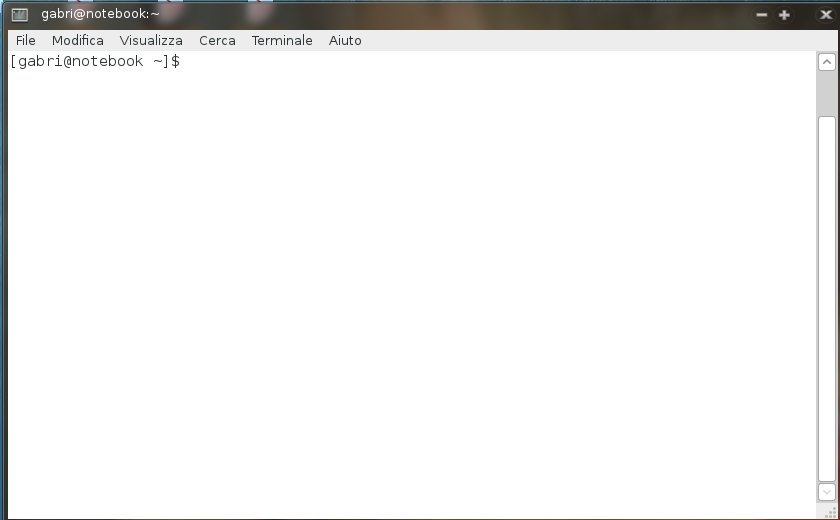
\includegraphics[scale=.30]{articoli/primi_passi/immagini/gnome_terminal.jpeg}
\caption{emulatore di terminale in Gnome (gnome terminal)\label{Fig.2: gnome_terminal}}
\end{figure}

\begin{center}
{\centering\bfseries La shell è entusiasmante}
\end{center}

Per chi arriva da altri sistemi operativi, dove l'interfaccia testuale è pressochè assente, si troverà spaesato di fronte alla necessità (talvolta assoluta) di dover aprire una shell per poter operare al meglio.\\

Dopo una normale diffidenza iniziale, in breve tempo avrà modo di apprezzare questo strumento basilare del sistema.\\

L'utente Linux è sempre spinto dalla curiosità e dalla voglia di capire ed è per questo che troverà molto piacevole appoggiarsi alla linea di comando.\\


\begin{figure*}[!htbp]
\centering
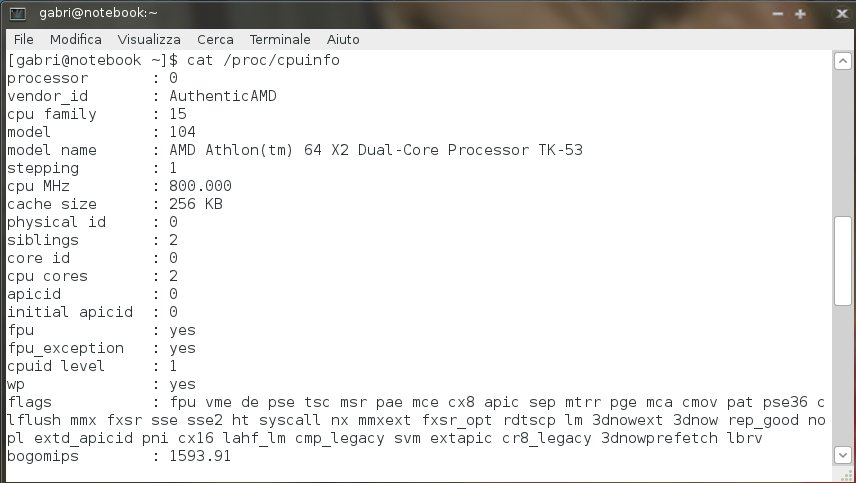
\includegraphics[scale=.60]{articoli/primi_passi/immagini/cpu_info.jpeg}
\caption{visualizzazione delle caratteristiche del processore in gnome-terminal\label{Fig.3: cpu_info}}
\end{figure*}


\begin{center}
{\bfseries La shell è potente}
\end{center}

A differenza delle interfacce grafiche, la shell permette una iterazione con il sistema molto elastica, arrivando in profondità fino ai processi vitali.\\

Tutto il sistema, con le dovute autorizzazioni, può essere modificato e analizzato per mezzo dei comandi e opzioni di programmi di utilità e software aggiuntivi.\\

Inoltre la shell è in grado di interpretare il proprio linguaggio di scripting ({\itshape bash scripting}) in cui la concatenazione di comandi e operatori può dare modo all'utente di automatizzare la propria attività.\\

\begin{center}
{\bfseries La shell non accetta la troppa confidenza}
\end{center}
Proprio per le qualità di cui sopra, corriamo il rischio di acquisire troppa confidenza con uno strumento che, a causa della sua caratteristica di iterazione anche a basso livello con il sistema, potrebbe indurci all'esecuzioni di operazioni senza la giusta dose di attenzione.\\

Si può arrivare a causare danni irreversibili alla propria station causando, spesso, perdite di dati, costringendoci ad un difficile recupero.\\

Non esiste un equilibrio oggettivo per questi fattori, il tutto è riconducibile alle proprie caratteristiche personali; di certo non bisogna temere il terminale ma sicuramente occorre avvicinarsi con piena coscienza di ciò che ci si accinge a fare.\\

Quindi il terminale ci consente di capire come funziona la nostra workstation ma, soprattutto, entriamo in sintonia con essa perchè ci permette di capire cosa stiamo facendo e cosa fa il sistema in risposta al nostro comando.\\

Chi ha acquisito una buona manualità sostiene che con il terminale si lavora molto velocemente; e non lo dicono solo i ``vecchi'' utilizzatori.\\

Aprendo la shell la riga che compare ({\itshape [gabri@notebook $\sim$]\textdollar}) è già fonte di alcune informazioni come il mio nome utente (gabri), il nome della mia macchina (notebook), in quale directory sono posizionato (la tilde $\sim$ indica che mi trovo all'interno della mia home, ovvero /home/gabri) ed infine il simbolo del dollaro (\textdollar), da distinguere da quello del cancelletto (\#) che sta a significare che ho acquisito le credenziali di root (quest'ultimo caso verrà trattato successivamente).\\

A questo punto il terminale è pronto ad accettare i comandi che vengono impartiti da tastiera.

\begin{figure*}[!t]
\centering
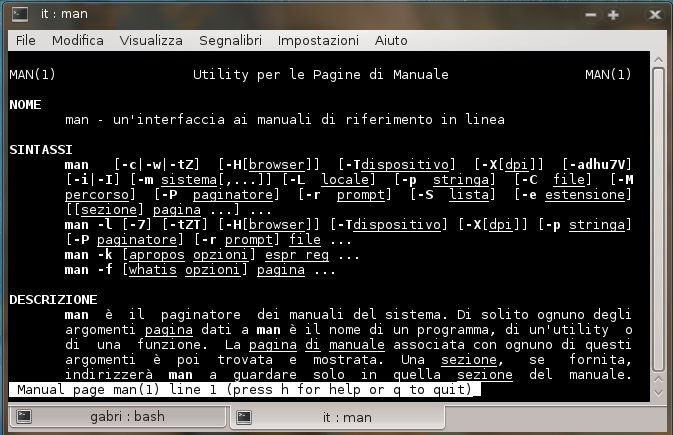
\includegraphics[scale=.80]{articoli/primi_passi/immagini/man_man.jpeg}
\caption{visualizzazione della pagina di manuale del comando {\itshape man}\label{Fig.4: man_man}}
\end{figure*}

\begin{shaded}
{\color[cmyk]{0, 0, 0, 0}\textdollar\ man nomecomando}
\end{shaded}
Utilizzando il comando qui sopra, appare all'interno del terminale virtuale il manuale di istruzione per l'utilizzo del comando dato come argomento; è sempre bene studiarlo per destreggiarsi nell'esecuzione secondo le nostre aspettative.\\

Già l'abituarsi alla lettura delle pagine {\itshape man} è un ottimo inizio, ma sicuramente il poter finemente configurare l'applicazione del comando mediante le opzioni rende molto interessante l'utilizzo della linea di comando.\\

Ovviamente il consiglio è quello di cimentarsi in esperimenti con comandi che non possono causare danni al sistema (come il comando {\itshape ls} oppure {\itshape cat} oppure lo stesso {\itshape man}), sebbene, utilizzando come utente e non come superuser, tali danni sarebbero circoscritti alla sola {\itshape /home} dell'utente stesso.\\

La {\itshape Bash} è inoltre fornita di completamento automatico; ci basta scrivere le lettere di inizio del comando per avere, premendo due volte il tasto {\itshape tab}, l'elenco completo dei comandi che iniziano con quelle lettere che ho premuto.\\
E' possibile, inoltre, usare la {\itshape history} per ripercorrere ed eventualmente selezionare gli ultimi comandi dati mediante l'utilizzo dei tasti ``freccia su'' e ``freccia giù''.\\

Da linea di comando è possibile anche avviare i programmi, anche quelli grafici, semplicemente inserendo il nome dell'eseguibile prima dell'invio:

\begin{shaded}
{\color[cmyk]{0, 0, 0, 0}\textdollar\ eseguibile}
\end{shaded}

come in questo caso specifico in cui lanciamo il web browser {\itshape firefox}, senza opzioni:

\begin{shaded}
{\color[cmyk]{0, 0, 0, 0}\textdollar\ firefox}
\end{shaded}

L'avvio dell'applicazione da terminale è utile soprattutto per un primo debug nel caso di malfunzionamento del lanciatore grafico, che invece non darebbe alcuna informazione aggiuntiva (l'applicazione non partirebbe e basta), mentre l'errore che viene segnalato in output è fondamentale per poter circostanziare il problema.\\

Autenticandoci come utenti, abbiamo delle restrizioni per quanto concerne la modifica o anche solo la visualizzazione dei file di sistema, proprio per evitare che, accidentalmente o meno, possa venire compromessa l'operatività della nostra stazione di lavoro.\\

Per interagire appieno occorre pertanto avere le credenziali del {\itshape superuser} (utente {\itshape root} che invece gode dei più ampi permessi.\\

Per diventare utente root occorre digitare al prompt:
\begin{shaded}
{\color[cmyk]{0, 0, 0, 0}\textdollar\ su}
\end{shaded}
e ci verrà richiesta la password assegnata all'utente root che, una volta inserita, ci permette di avere quei permessi necessari per l'amministrazione del sistema.

Da notare che, per motivi di sicurezza, alla digitazione della password di autenticazione, non si vedrà il cursore e che il prompt, come detto in precedenza, riporta il simbolo del cancelletto (\#).

\begin{figure}[!ht]
\centering
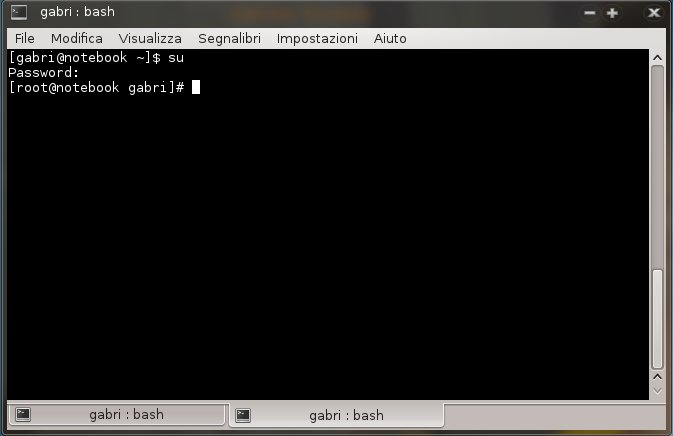
\includegraphics[scale=.35]{articoli/primi_passi/immagini/root.jpeg}
\caption{autenticazione di root}
\end{figure}

Eccoci autenticati come root nell'ambiente dell'utente (l'autenticazione con l'importazione dell'ambiente di root sarà oggetto di prossimi approfondimenti).\\

\hfill {\itshape (fine prima parte)}
\clearpage
\twocolumn[
\begin{center}
\title{\color[cmyk]{1, 0.57, 0, 0.38}{\Huge\bfseries Servizi di sistema (demoni)\\}} % definisco il titolo dell'articolo
\author{\scriptsize Gabriele Trombini (mailga@fedoraonline.it)} % definisco l'autore e altre informazioni
\date{}
\end{center}
{\color[cmyk]{1, 0.46, 0, 0}\LARGE (Parte prima) I servizi in Fedora - introduzione}\\
\maketitle
\normalsize
\doublespacing
\hfill
]
\definecolor{shadecolor}{cmyk}{0, 0, 0, 0.8}
\onehalfspacing
\lettrine[lines=1, loversize=0.1, lraise=0.1]{\color[cmyk]{0.5, 0, 1, 0}\bfseries C}{}ominciamo a dare una occhiata al sistema di gestione dei servizi che recentemente ha cominciato a sostituire {\itshape SysVinit} ed {\itshape Upstart} nell'avvio e nella gestione dei servizi.\\

I collaboratori italiani del team di traduttori del Fedora Project hanno preparato la pagina wiki {\itshape https://fedoraproject.org/ wiki/Features/systemd/it} dove sono ben spiegati i vantaggi di questo sistema di gestione della sessione e del sistema.\\

\begin{figure*}[!htbp]
\centering
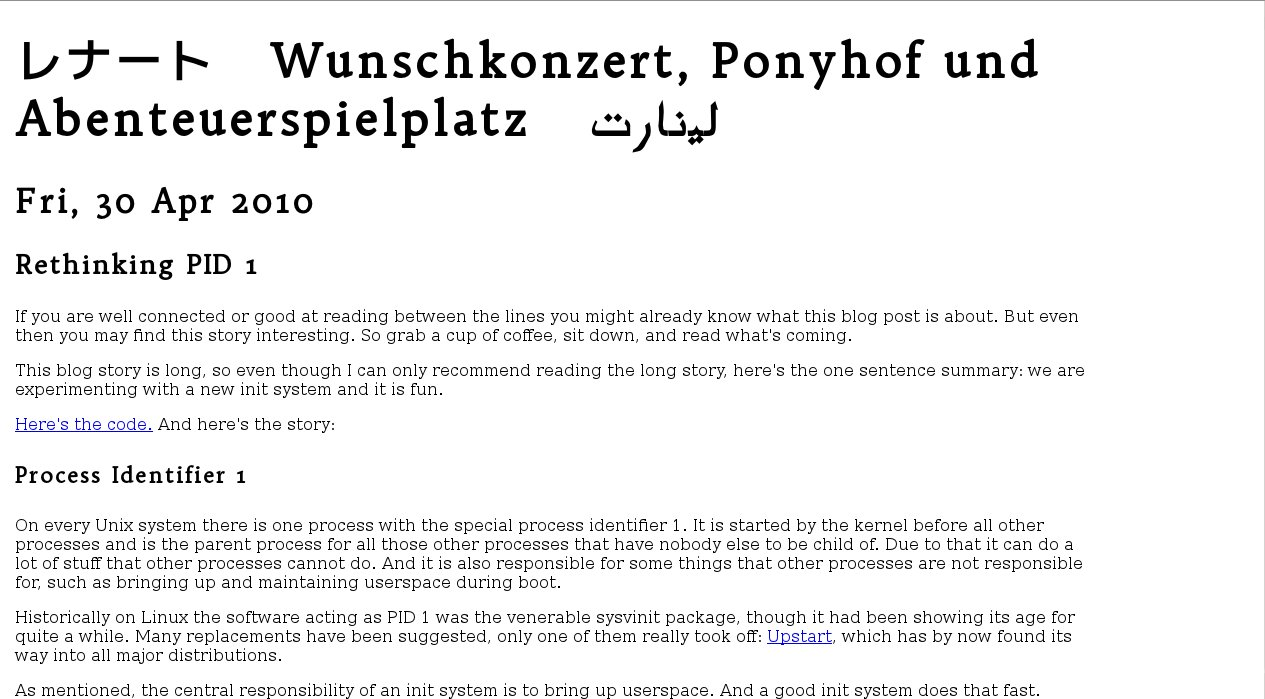
\includegraphics[scale=.45]{articoli/sistema_base/immagini/home_systemd.jpeg}
\caption{pagina del progetto ({\scriptsize http://0pointer.de/blog/projects/systemd.html})}
\end{figure*}

Facendo riferimento alla pagina del wiki\\{\itshape http://fedoraproject.org/wiki/Systemd},\\ dove troviamo dettagliatamente descritte le funzionalità, tra gli altri vantaggi notiamo che {\itshape systemd} velocizza l'avvio attivando processi in parallelo dando l'ascolto ai sockets prima di assegnare loro il servizio.\\

Il sistema {\itshape init} provvedeva a creare prima tutti i sockets e poi tutti i servizi, creando, in caso di dipendenza di un servizio rispetto ad un altro non ancora avviato, l'eventuale stallo del sistema o il mancato avvio del servizio stesso.\\

Inoltre esso si appoggia a D-Bus per l'avvio dei servizi on-demand, permette un recupero del sistema in caso di problemi (previo snapshot), si occupa del mount e dell'automount dei device (fstab può essere utilizzato come configurazione extra, indicando a {\itshape systemd} di monitorarlo), mantiene compatibilità con i sistemi precedenti e può essere configurato, praticamente, a piacimento.\\

Perciò, di fatto, a partire da Fedora 16 la nostra distribuzione ha introdotto in maniera massiva {\itshape systemd} per l'avvio e la gestione dei servizi.\\

Quali sono i vantaggi li abbiamo visti, seppur sommariamente (per approfondimenti dovremo studiarci le pagine web citate in precedenza), ma quello che più ci preme è la loro gestione.\\

Per facilitare il compito possiamo installare {\itshape systemadm} che ci fornisce una GUI con dei comandi minimali per l'avvio/ar\-resto/riavvio dei servizi, per esaminarli e per effettuare lo snapshot di cui sopra:

\begin{shaded}
{\color[cmyk]{0, 0, 0, 0}\#\ yum install systemd-gtk}
\end{shaded}
e per avviarlo: 
\begin{shaded}
{\color[cmyk]{0, 0, 0, 0}\textdollar\ systemadm}
\end{shaded}

Inutile dire che utilizzando il terminale possiamo fruire dei vantaggi della velocità di esecuzione uniti alle opzioni dei comandi.\\

Il tool testuale è {\itshape systemctl}, il cui utilizzo completo può essere studiato nelle pagine man:

\begin{shaded}
{\color[cmyk]{0, 0, 0, 0}\textdollar\ man systemctl}
\end{shaded}

\begin{figure*}[!htbp]
\centering
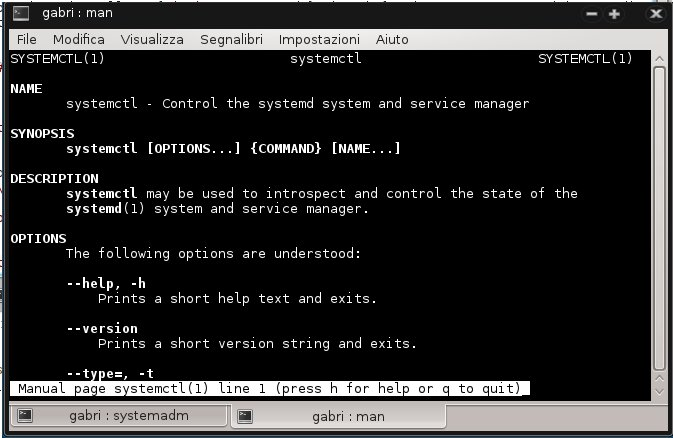
\includegraphics[scale=.80]{articoli/sistema_base/immagini/man_systemctl.jpeg}
\caption{pagina del manuale di systemctl}
\end{figure*}

Questo comando permette di effettuare tutte le principali operazioni di cui un utente potrebbe avere bisogno e la sintassi è molto semplice e, in qualche caso, ricorda l'utilizzo del comando ``service'', con il quale mantiene una certa compatibilità prima di essere totalmente abbandonato in futuro.
\begin{itemize}
\item verificare i servizi
\begin{shaded}
{\color[cmyk]{0, 0, 0, 0}\textdollar\ systemctl list-units --type=service}
\end{shaded}
\item verificare lo stato di un servizio
\begin{shaded}
{\color[cmyk]{0, 0, 0, 0}\textdollar\ systemctl status nome.service}
\end{shaded}
\item informazioni approfondite sullo stato di un servizio attivo
\begin{shaded}
{\color[cmyk]{0, 0, 0, 0}\textdollar\ systemctl is-active nome.service}
\end{shaded}
\item abilitare un servizio all'avvio
\begin{shaded}
{\color[cmyk]{0, 0, 0, 0}\#\ systemctl enable nome.service}
\end{shaded}
\item disabilitare un servizio all'avvio
\begin{shaded}
{\color[cmyk]{0, 0, 0, 0}\#\ systemctl disable nome.service}
\end{shaded}
\item avviare un servizio
\begin{shaded}
{\color[cmyk]{0, 0, 0, 0}\#\ systemctl start nome.service}
\end{shaded}
\item fermare un servizio
\begin{shaded}
{\color[cmyk]{0, 0, 0, 0}\#\ systemctl stop nome.service}
\end{shaded}
\item riavviare un servizio
\begin{shaded}
{\color[cmyk]{0, 0, 0, 0}\#\ systemctl restart nome.service}
\end{shaded}
\item ``uccidere'' un servizio
\begin{shaded}
{\color[cmyk]{0, 0, 0, 0}\#\ systemctl kill nome.service}
\end{shaded}
\end{itemize}

Cercando di andare un po' in profondità, possiamo vedere che le directory di riferimento di {\itshape systemd} sono fondamentalmente due:
\begin{itemize}
\item /etc/systemd
\item /lib/systemd 
\end{itemize}

Il contenuto della directory {\itshape /etc/systemd} ha la precedenza tra i due, ma entrambi contengono i servizi disponibili.\\

Ecco il file di configuraizone di mysqld:
\begin{shaded}
{\color[cmyk]{0, 0, 0, 0}[Unit]\\
Description=MySQL database server\\
After=syslog.target\\
After=network.target\\

[Service]\\
Type=forking\\
User=mysql\\
Group=mysql\\

ExecStartPre=/usr/libexec/mysqld-prepare-db-dir\\
\# Note: we set --basedir to prevent probes that might trigger SELinux alarms,\\
\# per bug \#547485\\
ExecStart=/usr/bin/mysqld\_safe --nowatch --basedir=/usr\\
ExecStartPost=/usr/libexec/mysqld-wait-ready \textdollar MAINPID\\

\# Give a reasonable amount of time for the server to start up/shut down\\
TimeoutSec=300\\

\# We rely on systemd, not mysqld\_safe, to restart mysqld if it dies\\
Restart=always\\
{\color[cmyk]{0, 0, 0, 0}[Unit]
[Install]\\
WantedBy=multi-user.target\\
}
}
\end{shaded}

Qualora volessimo creare un servizio, il file di configurazione deve essere inserito all'interno di {\itshape /lib/systemd}, e poi collegato in {\itshape /etc/systemd} così che alla variazione del primo, corrisponda la variazione del secondo.\\

 Per fare in modo che systemd venga a conoscenza del nuovo file:
\begin{shaded}
{\color[cmyk]{0, 0, 0, 0}\#\ systemctl systemctl daemon-reload}
\end{shaded}

Per abilitarlo all'avvio, basta quindi usare l'opzione --enable di cui abbiamo già parlato.\\

L'argomento merita un approfondimento maggiore (e per taluni aspetti ancora da scoprire) rispetto a quanto è possibile fare in un unico numero, tuttavia per un primo approccio al nuovo sistema di gestione dei servizi questo articolo può essere sufficiente.\\

Systemd verrà probabilmente ripreso nei prossimi numeri ad un livello di dettaglio più analitico, con esempi e con la chiamata in causa di {\itshape D-Bus}.\\


\hfill {\itshape (fine prima parte)}





\clearpage
\twocolumn[
\begin{center}
\title{\color[cmyk]{1, 0.57, 0, 0.38}{\Huge\bfseries Dracut \\}} % definisco il titolo dell'articolo
\author{\scriptsize Gabriele Trombini (mailga@fedoraonline.it)} % definisco l'autore e altre informazioni
\date{}
\end{center}
{\color[cmyk]{1, 0.46, 0, 0}\LARGE L'initramfs all'avvio di Fedora}\\
\maketitle
\normalsize
\doublespacing
\hfill
]
\definecolor{shadecolor}{cmyk}{0, 0, 0, 0.8}
\onehalfspacing
\lettrine[lines=1, loversize=0.1, lraise=0.1]{\color[cmyk]{0.5, 0, 1, 0}\bfseries C}{}ome sappiamo initrd e initramfs (per comodità diciamo che quest'ultimo è la versione attuale del precedente) non sono altro che dei file systems temporanei, che si collocano nella memoria, usati per caricare e montare il file system reale nel sistema.\\

Per compatibilità con un sistema generico, vengono inseriti al boot parecchi moduli di periferica e di filesystem ed il kernel, aumentando nelle dimensioni e nella quantità di hardware riconosciuto, impiega più tempo a caricarsi perciò si è reso necessario trovare soluzioni che mantengano un tempo ragionevole di start up.\\

A questo scopo è stata introdotta una fase iniziale di root file system in user space che si occupa di rilevare hardware, configurazioni, moduli prima di montare il file system root della macchina.\\

Difatti oggi la sequenza boot ordinariamente utilizzata è in due stages:
\begin{itemize}
 \item lancio e caricamento kernel con tutti i suoi moduli built-in ovvero i moduli integrati che sono indispensabili al corretto funzionamento di una macchina "base"
\item lancio di initramfs. Esso è di fatto un "micro sistema in ram" con le directory {\itshape bin - dev - etc- lib - tmp - var} etc... che provvede al caricamento non solo dei moduli atti al montaggio dei filesystem  e quindi del filesystem root, cosa fondamentale, ma anche al montaggio di altri moduli quali ad esempio gli alsa, quelli video (se necessario), con eventuali regole udev su determinati dispositivi, o altri moduli o performance che l'utente (esperto) decide di caricare subito con la modifica di {\itshape /etc/dracut.conf} o con l'inserimento di regole specifiche in {\itshape /etc/dracut.conf.d/}.
\end{itemize}

Dracut è quindi lo strumento che permette alla initial ramdisk di caricare solo quello che è necessario per l'avvio, creando una initramfs adatta al proprio sistema.\\

Tutto ciò avviene in automatico ma, qualora si avessero delle necessità particolari dovute ad installazioni successive di hardware o a moduli non interpretati dal sistema, è possibile utilizzare la linea di comando per effettuare le operazioni di creazione, variazione, verifica e manutenzione della inintramfs.\\

Il comando generico per poter creare un nuovo file system iniziale è:
\begin{shaded}
{\color[cmyk]{0, 0, 0, 0}\# dracut /boot/initramfs-\textdollar(uname -r).img \textdollar(uname -r)}\\
\end{shaded}

che viene utilizzato, ad esempio, dopo l'installazione dei driver grafici per poterli inserire già nel file system iniziale permettendo una corretta visualizzazione. \\

Come sempre in questi casi occorre sempre leggere il manuale dell'applicazione:

\begin{shaded}
{\color[cmyk]{0, 0, 0, 0}\textdollar\ man dracut}
\end{shaded}

all'interno del quale possiamo reperire le istruzioni e le opzioni per creare una immagine ramdisk iniziale integrando o escludendo moduli, filesystems, file di configurazione (compreso quello di deafult di dracut che è {\itshape /etc/dracut.conf}), partizioni e altro.\\

E' anche previsto un file di log, conseguente all'utilizzo di dracut, che trova posto all'interno della
directory {\itshape /var/log}, sotto il nome di {\itshape dracut.log}.

\begin{shaded}
{\color[cmyk]{0, 0, 0, 0}\textdollar\ cat  /var/log/dracut.log}
\end{shaded}

E' possibile inserire i parametri anche da linea di comando come descritto nella
pagina man:

\begin{shaded}
{\color[cmyk]{0, 0, 0, 0}\textdollar\ man dracut.kernel}
\end{shaded}

dove vediamo anche opzioni da passare al kernel all'avvio; conosciute ai più attenti perchè utilizzate anche nel grub.cfg di Fedora.\\

Può essere interessante guardare all'interno del file della initramfs utilizzando il tool {\itshape lsinitrd}
che ne permette l'ispezione:

\begin{shaded}
{\color[cmyk]{0, 0, 0, 0}\# lsinitrd /boot/initramfs-\textdollar(uname -r).img | more}
\end{shaded}

oppure verificare la presenza e contenuto di uno specifico file:

\begin{shaded}
{\color[cmyk]{0, 0, 0, 0}\# lsinitrd /boot/initramfs-\textdollar(uname -r).img run/initramfs/shutdown}
\end{shaded}

I file di configurazione di Dracut, in Fedora, devono essere posizionati all'interno della directory {\itshape /etc/dracut.conf.d/}, mentre il file da poter adattare alle proprie esigenze, commentandone e/o decommentandone le opzioni per meglio rifinire l'avvio, è {\itshape /etc/dracut.conf}.

\begin{shaded}
{\color[cmyk]{0, 0, 0, 0}\textdollar man dracut.conf}
\end{shaded}

Quanto inserito in {\itshape /etc/dracut.conf.d/} , in ordine numerico, va a sovrascrivere le impostazioni di {\itshape /etc/dracut.conf}, che invece è il file di prima lettura di dracut.\\

La particolarità di Dracut è data dal fatto che, proprio per adattare la singola macchina alle proprie necessità, si possa personalizzare la initramfs.\\

Utilizzando l'opzione {\itshape--include}, infatti, si possono inserire all'interno della initramfs i propri file di utilità particolare, ad esempio con il comando:

\begin{shaded}
{\color[cmyk]{0, 0, 0, 0}\# dracut --include /bin/cat / run/initramfs/usr/sbin initramfs-cat.img}
\end{shaded}
è possibile insterire il comando cat all'interno della directory {\itshape run/initramfs/usr/sbin} della initial ramdisk.\\

L'opzione {\itshape --install} consente di poter specificare diversi eseguibili che dovessimo ritenere utili all'avvio, rilevando anche le relative dipendenze:

\begin{shaded}
{\color[cmyk]{0, 0, 0, 0}\# dracut --install 'nmap ssh' initramfs-rete.img}
\end{shaded}

Vale la pena, anche, di ricordare che Dracut ha accesso ad una CLI, da dove si può cercare di fare un avvio manuale del sistema.\\

Togliendo  {\itshape rhgb} e {\itshape quiet} ed aggiungendo {\itshape rdshell} alle opzioni del kernel, si avrà a disposizione una shell con la quale cercare di eseguire il boot (per poi, magari, ricostruire la initial ramdisk una volta autenticati).\\

Tra i parametri utili per una analisi del sistema avremo a disposizione:

\begin{itemize}
 \item {\itshape rdshell}: come detto, inserendo questo comando si avrà accesso ad una shell di Dracut;
 \item {\itshape rdinitdebug}: per un livello di debug più approfondito, con stampa dei comandi;
 \item {\itshape rdbreak=[pre-udev | pre-mount | mount | pre-pivot |]}: aggiungendo questo parametro, la shell si fermerà prima di superare il punto dato come argomento;
 \item {\itshape rdudevinfo}: imposta udev ad un livello informativo massimo;
 \item {\itshape rdudevdebug}: imposta udev ad un livello di debug;
 \item {\itshape rdnetdebug}: verifica le connessioni network, l'output viene inserito in /tmp.
\end{itemize}

Questa breve panoramica non ha certo la pretesa di essere esaustiva ma quanto detto in questo articolo può concedere ampi spazi di approfondimento ai lettori.\\

\clearpage
\twocolumn[
\begin{center}
\title{\color[cmyk]{1, 0.57, 0, 0.38}{\Huge\bfseries Creazione di RPM \\}} % definisco il titolo dell'articolo
\author{\scriptsize Gabriele Trombini(mailga@fedoraonline.it)} % definisco l'autore e altre informazioni
\date{}
\end{center}
{\color[cmyk]{1, 0.46, 0, 0}\LARGE (Parte prima) RPM - introduzione}\\
\maketitle
\normalsize
\doublespacing
\hfill
]
\definecolor{shadecolor}{cmyk}{0, 0, 0, 0.8}
\onehalfspacing
\lettrine[lines=1, loversize=0.1, lraise=0.1]{\color[cmyk]{0.5, 0, 1, 0}\bfseries c}{}on l'acronimo {\itshape rpm} (RedHat Package Manager) si identifica sia il formato dei pacchetti usati da Fedora che l'utility per la loro gestione.\\

A dire il vero, seppur nato da Red Hat, questo formato riscosse fin dall'inizio un grande successo (al pari del formato .deb usato da debian e derivate), tant'è che ancora oggi viene utilizzato da altre distribuzioni (come Mandriva e Opensuse, inizialmente derivate da Red Hat) per l'installazione degli applicativi.\\

Lo stesso Fedora Project ne ha adottato lo standard come riferimento.\\

Malgrado vi siano diversi tools (come alien o checkinstall, anche se quest'ultimo non ha avuto nuove versione dal 2009) che permettono la creazione di {\itshape rpm}, con questo articolo vogliamo seguire le specifiche del Fedora Project riguardanti la creazione di un pacchetto dal punto di vista di un collaboratore packager, così come specificato all'indirizzo {\itshape http://fedo\\raproject.org/wiki/ Packaging:Guidelines}, tralasciando quindi le modalità di gestione, manutenzione e ispezione dei pacchetti mediante l'utilizzo del comando rpm e relative opzioni\\

Le linee guida sono molto dettagliate ed è consigliabile seguirle analiticamente in modo particolare qualora si volesse contribuire al progetto o mantenere i pacchetti di Fedora.

\begin{center}
{\bfseries Preparazione}
\end{center}

Come prima cosa è indispensabile che gli strumenti necessari alla corretta esecuzione delle operazioni siano installati sul propro computer:

\begin{shaded}
{\color[cmyk]{0, 0, 0, 0}\# yum install @Strumenti$\backslash$ di$\backslash$ sviluppo}
\end{shaded}

\begin{shaded}
{\color[cmyk]{0, 0, 0, 0}\# yum install fedora-packager}
\end{shaded}

Quest'ultimo comando installa come dipendenza anche l'utility {\itshape rpmdevtools} che ci consente di utilizzare il comando adatto alla creazione dell'albero per lo sviluppo:

\begin{shaded}
{\color[cmyk]{0, 0, 0, 0}\$ rpmdev-setuptree}
\end{shaded}

Al termine del comando possiamo controllare che nella home dell'utente in uso sia presente la cartella rpmbuild, che a sua volta contiene altre directory (al momento vuote).

\begin{figure*}[!ht]
\centering
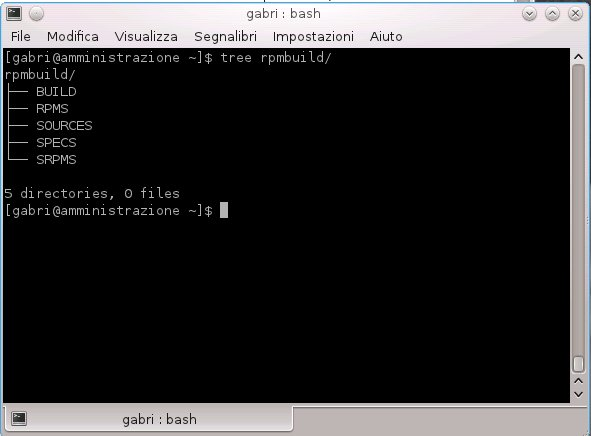
\includegraphics[scale=.95]{articoli/sistema_avanzato/immagini/rpmbuild_tree.jpeg}
\caption{l'albero di sviluppo dei pacchetti }
\end{figure*}

\begin{itemize}
\item SOURCES — dove devono essere inseriti i file sorgenti, le patch ed i file di icone;
\item SPECS — dove devono essere inseriti i file .spec;
\item BUILD — dove i sorgenti saranno scompattati ed il pacchetto costruito;
\item RPMS — dove il processo build inserirà il pacchetto binario;
\item SRPMS — dove il processo build inserirà il pacchetto sorgente.
\end{itemize}

A questo punto tutto è pronto per cominciare il nostro lavoro di packaging ma, se vogliamo essere conformi a quanto previsto dal Fedora Project, è bene che si legga in particolare le specifiche riguardanti:

\begin{enumerate}
\item nomenclatura ({\itshape http://fedoraproje\\ct.org/wiki/Packaging:NamingGui\\delines\ \#Package\_Naming\_and\_\\Versioning\_Guidelines});
\item versione e release ({\itshape http://fedora\\project.org/wiki/Packaging:Nami\\ngGuidelines\#Package\_Version});
\item aspetti legali ({\itshape https://fedoraproje\\ct.org/wiki/Packaging/Guidelines\#\\Legal});
\item licenza ({\itshape http://fedoraproject.org\\/wiki/Packaging:LicensingGuideli\\nes});
\end{enumerate}

Oltre a quanto sopra, occorre tenere presente anche altri aspetti, di carattere più pratico, legati alla preparazione dei pacchetti per la nostra distribuzione.\\
 
\begin{itemize}
\item tutto il software presente deve essere libero ed opensource;
\item le inclusioni devono essere inserite partendo dai sorgenti;
\item non costruire i pacchetti utilizzando l'utente root (è possibile creare un utente per lo sviluppo);
\item seguire le direttive di layout del FHS (Filesystem Hierarchy Standard) che definisce come devono essere distribuiti i file nel sistema e, se si dovesse avere necessità di creare nuove directory, è bene chiedere, motivando l'operazione, al Fedora Packaging Committee;
\item non inserire file in /bin, /sbin, /lib or /lib64, bensì utilizzare /usr/bin, /usr/sbin, /usr/lib, and /usr/lib64 (è possibile usare dei link simbolici a queste directory);
\end{itemize}

Come già detto Il Fedora Packaging Committee può rispondere ad eventuali dubbi.\\

\begin{figure}[!ht]
\centering
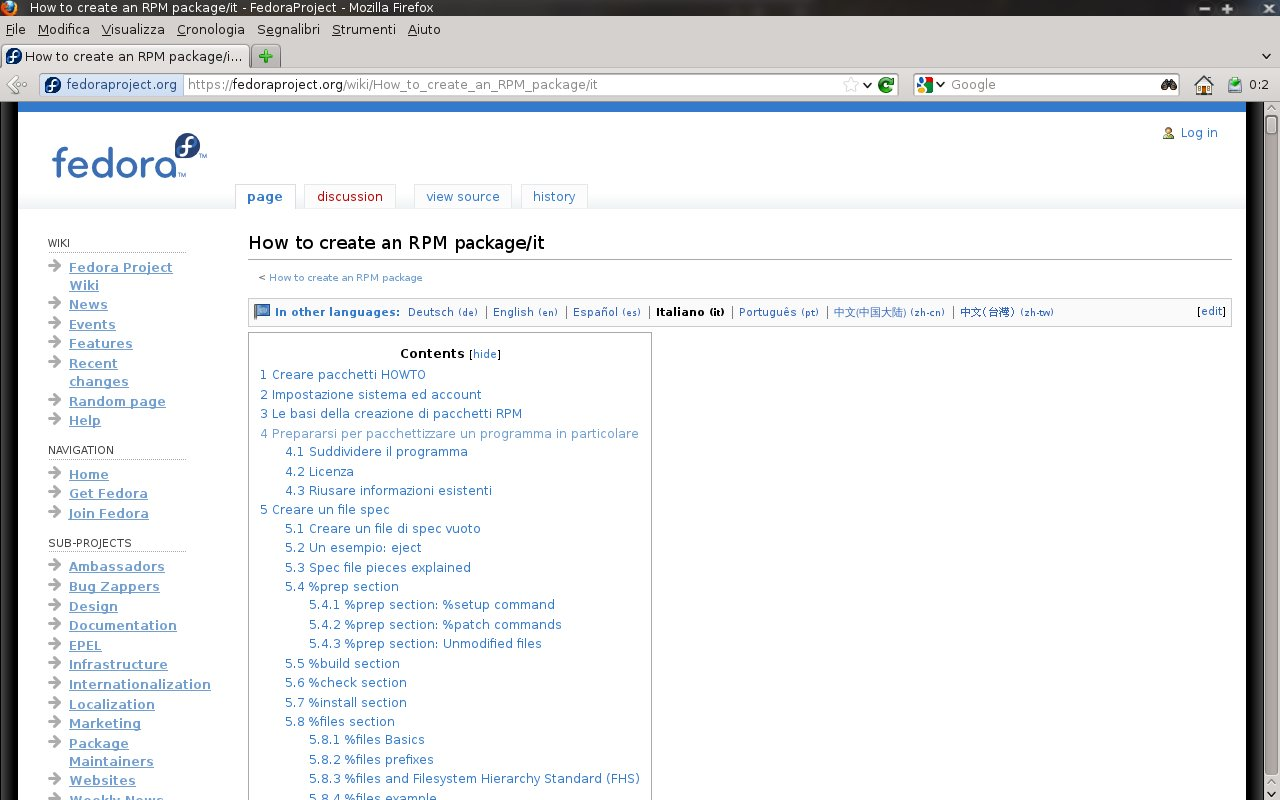
\includegraphics[scale=.21]{articoli/sistema_avanzato/immagini/rpm_wiki.jpeg}
\caption{come creare un rpm, la pagina tradotta dal team italiano}
\end{figure}

Arrivati a questo punto abbiamo preparato il nostro sistema per il packaging e siamo pronti ad eseguire il processo secondo le indicazioni del Progetto Fedora.\\

Il passo successivo che vedremo nel prossimo numero, sarà quello di creare il file {\itshape .spec}, un fondamentale file di testo contenente le informazioni necessarie alla pacchettizzazione dell'applicativo.\\


\hfill {\itshape (fine prima parte)}


\begin{comment}
Il primo passaggio da considerare è dato dal file .spec, un semplice file di testo contenente le informazioni necessarie alla pacchettizzazione dell'applicativo.

Fasi dell'rpmpbuild:

Nome della Macro 	Nome 	Di solito 	Scopo
%_specdir	directory della Specifica	~/rpmbuild/SPECS	file di specifica RPM (.spec)
%_sourcedir	directory Source	~/rpmbuild/SOURCES	Pacchetto dei sorgenti incontaminati (es: tarballs) e patch
%_builddir	Build directory	~/rpmbuild/BUILD	Source files are unpacked and compiled in a subdirectory underneath this.
%_buildrootdir	directory root di Build 	~/rpmbuild/BUILDROOT	I file vengono installati qui durante la fase %install.
%_rpmdir	directory dei binari RPM directory	~/rpmbuild/RPMS	Binari RPM sono creati e immagazzinati qui sotto.
%_srcrpmdir	directory dei Sorgenti RPM	~/rpmbuild/SRPMS	Il sorgente RPM sono creati e immagazzinati qui sotto. 

Creare un file spec

E' necessario creare ora il file ".spec" nella directory "~/rpmbuild/SPECS". E' consigliato dare al file il nome del programma, es: "programma.spec". Usa il nome dell'archivio oppure il nome sostenuto dall'autore del programma dove possibile, ma assicurati di rispettare le Linee guida per il Naming dei pacchetti.
Creare un file di spec vuoto

Quando crei uno spec file per la prima volta, è possibile usare la versione iniziale emacs o vim (dalla 7.1.270-1) che creano automaticamente un template per voi, ES.:

 $ cd ~/rpmbuild/SPECS
 $ vi program.spec

Di seguito un esempio di questo template:

Name:		
Version:	
Release:	1%{?dist}
Summary:	
Group:		
License:	
URL:		
Source0:	
BuildRoot:	%{_tmppath}/%{name}-%{version}-%{release}-root-%(%{__id_u} -n)

BuildRequires:	
Requires:	

%description

%prep
%setup -q

%build
%configure
make %{?_smp_mflags}

%install
rm -rf %{buildroot}
make install DESTDIR=%{buildroot}

%clean
rm -rf %{buildroot}

%files
%defattr(-,root,root,-)
%doc

%changelog


Puoi avere $RPM_BUILD_ROOT al posto di %{buildroot}; basta che sia consistente.

Puoi usare il comando rpmdev-newspec per creare un file di spec per te. rpmdev-newspec NOME-DEL-NUOVO-PACCHETTO crea un file spec iniziale per un nuovo pacchetto, su misura per vari tipi di pacchetti. Il programma individuerà il tipo di template da usare dal nome del pacchetto, o puoi specificare un particolare tipo di modello; controlla /etc/rpmdevtools/spectemplate-*.spec per consultare i template disponibili. Controlla rpmdev-newspec --help per maggiori informazioni. Per esempio, per creare un nuovo file di spec per un modulo python:

cd ~/rpmbuild/SPECS
rpmdev-newspec python-antigravity
vi python-antigravity.spec

Un esempio: eject

Di seguito un esempio, un pacchetto per Fedora 9 per il programma "eject":

Summary: A program that ejects removable media using software control
Name: eject
Version: 2.1.5
Release: 11%{dist}
License: GPL
Group: System Environment/Base
Source: http://metalab.unc.edu/pub/Linux/utils/disk-management/%{name}-%{version}.tar.gz
Source1: eject.pam
Patch1: eject-2.1.1-verbose.patch
Patch2: eject-timeout.patch
Patch3: eject-2.1.5-opendevice.patch
Patch4: eject-2.1.5-spaces.patch
Patch5: eject-2.1.5-lock.patch
Patch6: eject-2.1.5-umount.patch
BuildRoot: %{_tmppath}/%{name}-%{version}-%{release}-root
URL: http://www.pobox.com/~tranter
ExcludeArch: s390 s390x
BuildRequires: gettext
BuildRequires: automake
BuildRequires: autoconf
BuildRequires: libtool

%description
The eject program allows the user to eject removable media (typically
CD-ROMs, floppy disks or Iomega Jaz or Zip disks) using software
control. Eject can also control some multi-disk CD changers and even
some devices' auto-eject features.

Install eject if you'd like to eject removable media using software
control.

%prep
%setup -q -n %{name}
%patch1 -p1 -b .versbose
%patch2 -p1 -b .timeout
%patch3 -p0 -b .opendevice
%patch4 -p0 -b .spaces
%patch5 -p0 -b .lock
%patch6 -p1 -b .umount

%build
%configure
make

%install
rm -rf %{buildroot}

make DESTDIR=%{buildroot} install

# pam stuff
install -m 755 -d %{buildroot}/%{_sysconfdir}/pam.d
install -m 644 %{SOURCE1} %{buildroot}/%{_sysconfdir}/pam.d/%{name}
install -m 755 -d %{buildroot}/%{_sysconfdir}/security/console.apps/
echo "FALLBACK=true" > %{buildroot}/%{_sysconfdir}/security/console.apps/%{name}

install -m 755 -d %{buildroot}/%{_sbindir}
pushd %{buildroot}/%{_bindir}
mv eject ../sbin
ln -s consolehelper eject
popd

%find_lang %{name}

%clean
rm -rf %{buildroot}

%files -f %{name}.lang
%defattr(-,root,root)
%doc README TODO COPYING ChangeLog
%attr(644,root,root) %{_sysconfdir}/security/console.apps/*
%attr(644,root,root) %{_sysconfdir}/pam.d/*
%{_bindir}/*
%{_sbindir}/*
%{_mandir}/man1/*

%changelog
* Wed Apr 02 2008 Zdenek Prikryl <zprikryl at, redhat.com> 2.1.5-11
- Added check if device is hotpluggable
- Resolves #438610



    Name: The (base) name of the package. It must follow the Package Naming Guidelines. In many cases, this will be in all lower case. Elsewhere in the spec file, you can refer to the name using the macro %{name} - that way, if the name changes, the new name will be used by those other locations. This name should match the spec file name.
    Version: The upstream version number. See Packaging/Naming guidelines - package version for more information. If the version is non-numeric (contains tags that are not numbers or digits), you may need to include the additional non-numeric characters in the release field. If upstream uses full dates to distinguish versions, consider using version numbers of the form yy.mm[dd] (so a 2008-05-01 release becomes 8.05). Elsewhere in the spec file, refer to this value as %{version}.
    Release: The initial value of the release should normally be "1%{?dist}". Then, increment the number every time you release a new package for the same version of software. If a new version of the software being packaged is released, the version number should be changed to reflect the new software version, and the release number should be reset to 1. See Name Guidelines - package release for more. Packaging/DistTag describes the "dist" tag, which isn't required but can be useful. Use %{release} to reuse this value.
    Summary: A brief, one-line summary of the package. Use American English, and do not end in a period.
    Group: This needs to be a pre-existing group, like "Applications/Engineering"; run "less /usr/share/doc/rpm-*/GROUPS" to see the complete list. If you create a sub-package "...-doc" with documentation, use the group "Documentation".
    License: Its license; for software, this must be an open source software license. Use a standard abbreviation, e.g., "GPLv2+". Try to be specific, e.g., use "GPLv2+" (GPL version 2 or greater) instead of just "GPL" or "GPLv2" where it's true. See Licensing and the Licensing Guidelines for more information. You can list multiple licenses by combining them with "and" and "or", e.g., "GPLv2 and BSD". Call this tag "License"; don't use the older, inaccurately named tag "Copyright".
    URL: The URL for more information about the program, e.g., the project website. Note: This is NOT where the original source code came from, see "Source" (next!).
    Source0: The URL for the compressed archive containing (original) pristine source code, as upstream released it. "Source" is synonymous with "Source0". If you give a full URL (and you should), its basename will be used when looking in the SOURCES directory. If possible, embed %{name} and %{version}, so that changes to either will go to the right place. Warning: Source0: and URL: are different - normally they are both URLs, but the "URL:" entry points to the project website, while the "Source0:" entry points to the actual file containing the source code (and is typically a .tar.gz file). As noted in the guidelines, "When downloading sources, patches etc, consider using a client that preserves the upstream timestamps. For example wget -N or curl -R. To make the change global for wget, add this to your ~/.wgetrc: timestamping = on, and for curl, add to your ~/.curlrc: -R." If there is more than one source, name them Source1, Source2, and so on. If you're adding whole new files in addition to the pristine sources, you can list each of them as sources as well, but list them after the pristine sources. A copy of each of these sources will be included in any source package you create (unless you specially direct otherwise). See Packaging/SourceURL for more information on special cases (using revision control, when upstream uses prohibited code, etc.).
    Patch0: The name of the first patch that you will apply to the source code. If you need to patch the files after they've been uncompressed, you should edit the files, save their differences as a "patch" file in your ~/rpmbuild/SOURCES directory. Patches should make only one logical change, so it's quite possible to have multiple patch files.
    BuildArch: If you're packaging files that are architecture-independent (e.g., shell scripts, data files, etc.), then add "BuildArch: noarch". The architecture for the binary RPM will then be "noarch".
    BuildRoot: This is where files will be "installed" during the "%install" process (which happens after the %build compilation process). Normally you should just leave this line alone; under the usual Fedora setup, this will be a macro that will create a new special directory under /var/tmp. Newer versions of RPM will ignore this value, and instead place the build root in "%{_topdir}/BUILDROOT/".
    BuildRequires: A comma-separated list of packages required for building (compiling) the program. These are not automatically determined, so you need to include everything needed to build the program. There are a few packages that are so common in builds that you don't need to mention them, such as "gcc"; see the Packaging Guidelines for the complete list of the packages you may omit. You can also specify minimum versions, if necessary, like this: "ocaml >= 3.08". You can have more than one line of BuildRequires (in which case they are all required for building). If you need file /EGGS, you can get its package by running "rpm -qf /EGGS"; if EGGS is a program, you determine its package quickly by running "rpm -qf `which EGGS`". Try to specify only the minimal set of packages necessary to properly build the package, since each one will slow down a "mock"-based build (e.g., try to use sed instead of perl if you don't really need perl's abilities). Watch out: Some applications permanently disable functions if their package isn't detected during the build; in those cases you may need to include those additional packages. If you have trouble figuring out this list, the "auto-br-rpmbuild" command (from the auto-buildrequires package) may be helpful.
    Requires: A comma-separate list of packages that are required when the program is installed. Note that the list of packages for Requires (what's required when installing/running) and BuildRequires (what's required to build the binary RPM) are independent; a package may be in one list but not the other, or it could be in both. The dependencies of binary packages are in many cases automatically detected by rpmbuild, so it is often the case that you don't need to specify the Requires tag at all. But if you want to highlight some specific packages as being required, or require a package that rpm can't detect should be required, then add it here.
     %description - A longer, multi-line description of the program. Use American English. All lines must be 80 characters or less. "Blank lines are assumed to separate paragraphs. Some graphical user interface installation programs will reformat paragraphs... (lines that) start with whitespace, such as a space or tab, will be treated as preformatted text and displayed as is, normally with a fixed-width font." (per the RPM Guide).
     %prep - Script commands to "prepare" the program, that is, to uncompress it so that it will be ready for building (compiling). Typically this is just "%setup -q" or some variation of it; a common variation is "%setup -q -n NAME" if the source file unpacks into NAME. See the "%prep" section below for more.
     %build - Script commands to "build" the program, that is, to compile it and get it ready for installing. The program should come with instructions on how to do this. See the "%build" section below for more.
     %check - Script commands to self-test the program. This is run after %build and before %install, so you should place it there if you have this section. Often it simply contains "make test" or "make check". This is separated from %build so that people can skip the self-test if they desire. This isn't documented in many places.
     %install - Script commands to "install" the program. The commands should copy the files from the "build directory" %{_builddir} (which would be under ~/rpmbuild/BUILD) into the buildroot directory, %{buildroot} (which would normally be under /var/tmp). See the "%install" section below for more.
     %clean - instructions to clean out the build root. Typically: 

rm -rf %{buildroot}

     %files - the list of files that will be installed. See the "%files" section below for more.
     %changelog - Changes in the package. Use the format example above.
    ExcludeArch: If the package does not successfully compile, build or work on an architecture, then those architectures should be listed in the spec in an ExcludeArch tag.
    You can add sections so that code will run when packages are installed or removed on the real system (as opposed to just running the %install script, which only does a pseudo-install to the build root). These are called "scriptlets", and they are usually used to update the running system with information from the package. See the "Scriptlets" section below for more. 

Don't use the tags "Packager" or "Vendor". Don't use "Copyright" - use "License" instead. Don't create a "relocatable" package - they don't add value in Fedora yet they make things more complicated.

RPM supports subpackages, that is, a single spec file can generate many binary packages. For example, if the documentation is very large, you might generate a separate "-doc" subpackage. See below for more.
 %prep section

The "%prep" section describes how to unpack the compressed packages so that they can be built. Typically, this is a set of "%setup" and/or %patch commands, which reference the Source0:, Source1:, etc. lines above. See the Maximum RPM section on %setup and %patch for more details.

Warning: In spec files, don't use in-line comments (a "#" comment on the same line after a command), and don't put macros (words beginning with "%") in a comment unless you quote the "%" as "%%". Macros can cause failures if they are in a comment, because they are always expanded (even when in a comment) and they can expand to multiple lines. This is true for %prep, %build, and so on.

The new RPM 4.4.2.x series adds two new macros, %{patches} and %{sources}, so you can do things like:

for p in %{patches}; do
...
done

These new macros can be very useful if you have a large list of patches or sources. However, keep in mind that using these will make your spec incompatible with the rpm used in Fedora 9 and earlier, RHEL, and many other RPM-based distros.
 %prep section: %setup command

The "%setup" command unpacks a source package, and takes several switches. Normally you should use "-q" (quiet) to prevent setup from babbling about every file it unpacks. Here are a few switches besides -q:

    -n name: If the name of the rpm is something other than what the Source unpacks to, use this switch to state the name it unpacks to. E.G., if the tarball unpacks into a directory MYNAME, use %setup -q -n MYNAME
    -c name: If the tarball doesn't unpack into a single directory, this creates a directory named name and then unpacks into it. Useful if you have one of those annoying tarballs that doesn't have a single common subdirectory embedded in it. 

There are more %spec options if you are unpacking multiple files, which is primarily useful if you are creating subpackages (see below). The key ones are:
-a number 	Only unpack the source directive of the given number, such as –a 0 for source0:, after changing to the directory.
-b number 	Only unpack the source directive of the given number, such as –b 0 for source0:, before changing to the directory.
-D 	Do not delete the directory before unpacking.
-T 	Disable the automatic unpacking of the archives.
 %prep section: %patch commands

The "%patch0" command applies patch 0 (similar for 1, 2, etc.). Patches are the normal way to change to the source code if necessary to package it. The normal "-pNUMBER" option applies, which simply passes that argument on to patch.

Patch file names often look like "telnet-0.17-env.patch", that is, %{name}-%{version}-patch_purpose.patch (some people omit -%{version}). Patch files are typically the result of a "diff -u"; if you do this from the subdirectory of ~/rpmbuild/BUILD, you won't have to specify a -p level later. You can use all the normal ways of creating a patch file.

If you're creating a patch file a single file FILENAME, a common way is to copy it to FILENAME.orig, modify it, and then save the results of "diff -u FILENAME.orig FILENAME". If you change directory to "~/rpmbuild/BUILD/NAME", you could create a patch file to change a single file by doing:

cp X/Y.Z X/Y.Z.orig
vim X/Y.Z
diff -u X/Y.Z.orig X/Y.Z > ~/rpmbuild/SOURCES/PKGNAME.REASON.patch

If you're going to edit many files, one easy method is to copy the whole subdirectory underneath BUILD, and then do subdirectory diffs; once you change directory to "~rpmbuild/BUILD/NAME", you can:

cp -pr ./ ../PACKAGENAME.orig/
... many edits ...
diff -u ../PACKAGENAME.orig . > ~/rpmbuild/SOURCES/NAME.REASON.patch

If you edit many files in one patch, you can also copy the original files using some consistent ending such as ".orig" before editing them. Then, you can use "gendiff" (in the rpm package) to create a patch with the differences. Do "man gendiff" for more information.

Try to ensure that in your patch the "context" matches exactly. In old versions of Fedora, the default "fuzz" value was 2, which meant that imprecise matches were acceptable. However, the version of RPM used by Fedora 10 and later have a default fuzz to 0, requiring that matches be exact. You can work around this by adding "%global _default_patch_fuzz 2", but it's better to not have the problem by making the patch match the context exactly.

As explained in Packaging/PatchUpstreamStatus, all patches in Fedora spec files SHOULD have a comment above them about their upstream status. This should document the upstream bug/email that includes it (including the date), or if it's Fedora-unique, why it is unique. The Fedora Project focuses, as much as possible, on not deviating from upstream in the software it includes in the repository - see Staying close to upstream projects for more about why it's important to do this.
 %prep section: Unmodified files

Sometimes, you'll package just a straight file that doesn't need to be uncompressed, e.g., a "Source1:" that is just a simple PDF file. These might not be from external sources, e.g., perhaps you've had to create a few additional files that weren't in the original sources so that the package cleanly installs in Fedora. You can "prep" those into the build directory by doing this (replace "1" with whatever number it is):

 cp -p %SOURCE1 .

 %build section

The "%build" section is sometimes complicated; here you configure and compile/build the files to be installed.

Many programs follow the GNU configure approach (or some variation). By default, they will install to a prefix of "/usr/local" (/usr/local/bin, /usr/local/lib, etc.), which is a reasonable default for unpackaged files. However, since you are packaging it, you will want to change the prefix to "/usr", since this is now a package maintained by the system itself. If there are any libraries, they'll need to be installed in the right directory, which is either /usr/lib or /usr/lib64 depending on the architecture (the actual value is in %{_libdir}).

Since the GNU "configure" system is so common, rpm pre-defines a macro named "%configure", which invokes GNU configure with the right options (e.g., it changes --prefix to /usr). This means that some variation of this will often work as a build command:

 %configure
 make %{?_smp_mflags}

Sometimes you'll want to override the variables of a makefile; you can easily do that by passing them as parameters to make, like this:

make %{?_smp_mflags} CFLAGS="%{optflags}" BINDIR=%{_bindir}

If you need to do something complicated with GNU-generated configure, take a look at "GNU autoconf, automake, and libtool". A good presentation on these as well as "make" is "Open Source Development Tools: An Introduction to Make, Configure, Automake, Autoconf" by Stefan Hundhammer.

Some programs use Cmake. See Packaging/cmake for some suggestions.

If you include some self-tests (and that's a good idea), put them in a separate "%check" section that immediately follows the "%build" area, instead of including them in %build. That way, it will be easy for the system to skip unnecessary self-tests.
 %check section

The "%check" section does testing, often it's "make test". This is not documented in many other sources of RPM info.
 %install section

The "%install" section is a set of script commands to "install" the program. The commands in this section should copy the files from a directory inside the "build directory" %{_builddir} (normally ~/rpmbuild/BUILD/something) into the build root directory, %{buildroot} (normally /var/tmp/something), creating the directories inside %{buildroot} as necessary.

Watch out: Some of the terminology is very misleading:

    The build directory (under which compilations occur during %build) and the build root (where files are copied into during the %install process) are different. The point of the %install process is to copy files, such as those under the build directory, to the right place in the build root. Perhaps "buildroot" should be called "installroot", but it's too late now, the terminology is entrenched.
    The build directory is normally ~/rpmbuild/BUILD, while the build root (where files get installed to during %install) is normally ~/rpmbuild/BUILDROOT. The %prep stage will normally create a subdirectory underneath the build directory as part of %setup, and populate the build directory with files (based on the source information in %_sourcedir, which is typically in ~/rpmbuild/SOURCES). During %build, the current directory will actually start at %{buildsubdir}, that newly-created subdirectory under the build directory. Typically %{buildsubdir} is something like ~/rpmbuild/BUILD/%{name}-%{version}.
    The "%install" script is not used when the binary rpm package is installed by the end-user!! The term "%install" is misleading, in fact, the script must not install the programs in the REAL final locations (e.g., in /usr/bin), but under the buildroot %{buildroot}. 

Normally, the install script would first erase the %{buildroot} directory, and then do some variation of "make install" (ideally using DESTDIR=%{buildroot}, if the program supports it). Here's an example of an %install section:

%install
rm -rf %{buildroot}
make DESTDIR=%{buildroot} INSTALL="install -p" CP="cp -p" install

Ideally, every program would have a "make install" command that supported the DESTDIR convention. If the program includes a "make install" that supports DESTDIR, where possible, use it. The DESTDIR convention supports redirecting file installations to descend from a specific directory, which is exactly what we want during %install.

Installing a program that does not support DESTDIR can be much harder, and no option is as good as native DESTDIR support. Consider these alternatives:

    Patch the makefile so that it does support DESTDIR. Create directories inside DESTDIR where necessary (feel free to use "mkdir -p", the "-p" option of mkdir is now standard and widely supported). Be sure to submit the patch upstream.
    Use "%makeinstall". Many older RPM documents suggest using "%makeinstall", which might work if "make install" doesn't support DESTDIR. However, as noted in the Fedora guidelines, the %makeinstall macro "must NOT be used when make install DESTDIR=%{buildroot} works. %makeinstall is (merely) a kludge that can work with Makefiles that don't make use of the DESTDIR variable...". Unfortunately, this sometimes has subtle failures, which is why %makeinstall should not be used if DESTDIR works. The reason is based on how %makeinstall works. The "%makeinstall" macro expands to something like "make prefix=%{buildroot}%{_prefix} bindir=%{buildroot}%{_bindir} ... install". Many programs will quietly recompile or change parts of the program when values like prefix are changed, resulting in an incorrect installation. See the Fedora guidelines if you want the details on why this approach can fail. You will probably need to create appropriate directories inside %buildroot before calling %makeinstall (e.g., mkdir -p %{buildroot}%{_bindir}/).
    Consider using the auto-destdir package. This requires "BuildRequires: auto-destdir", and changing "make install" to "make-redir DESTDIR=%{buildroot} install". This only works well if the installation uses only certain common commands to install files, like cp and install; see "man make-redir" for details.
    Do the installation "by hand", that is, instead of invoking a build system, copy the files to the correct locations. Basically, this would be a sequence that would create directories that weren't already created by the "BuildRequires" packages (typically using install -d or mkdir -p), followed by copying of files from the current directory (inside the build directory) into the buildroot directory (typically using "cp -p" and/or "install -p"). Running "make -n install" may make it easy to determine what this sequence should be. Be sure to create directories inside %buildroot where necessary. One serious problem with this approach is that it's easy to fail to install new or renamed files during an update—so if there's a better approach, use it instead. If you do perform the installation "by hand", be especially careful with updates when using this approach. For example: 

%install
rm -rf %{buildroot}
mkdir -p %{buildroot}%{_bindir}/
cp -p mycommand %{buildroot}%{_bindir}/

As noted in the packaging guidelines' timestamp section, "when adding file copying commands in the spec file, consider using a command that preserves the files' timestamps, eg. cp -p or install -p". So, if the makefile lets you override the install command (typically named INSTALL), you might want something like INSTALL="install -p" CP="cp -p" as make parameters, like this:

make INSTALL="install -p" CP="cp -p" DESTDIR=%{buildroot} install

 %files section

The %files section identifies what files and directories were added by the package - and thus, which files and directories are owned by the package. Ownership is important - when you type "rpm -qif blah", you'll see who owns blah. This section is used when performing the bin stage, to determine which files are placed into each binary RPM file.
 %files Basics

The %files section normally begins with a %defattr line which sets the default file permissions. The format of this is %defattr(<file permissions>, <user>, <group>, <directory permissions>), that is, one can specify the permissions to apply to files and directories in the %files section. The fourth parameter is often omitted. Usually one uses %defattr(-,root,root,-), where "-" means "use the default permissions".

This is followed by names or patterns of the directories or files to be installed and owned by this package. You should use macros for directory names, e.g., use %{_bindir}/myfile instead of /usr/bin/myfile, and %{_sbindir}/killaccount instead of /usr/sbin/killaccount. If a name or pattern begins with "/" when expanded, then it is presumed to have been copied into the %{buildroot} followed by that pattern; when installed on the final system, it will be copied into that name without the buildroot prefix. If you don't precede the pattern with "/", then it is presumed to be in the current directory (e.g., inside the build directory) - this is used for "documentation" files. So if your package just installs /usr/sbin/mycommand, then your %files section could simply say:

%files
%defattr(-,root,root,-)
%{_sbindir}/mycommand

Any file or directory identified in the %files section is owned by the defining package. You should make sure that you declare ownership of every new file or directory the package creates. You can use wildcards (*) which match a set of files - this makes the package less sensitive to changes. For example, you can declare that all the files that were copied into %{buildroot}/usr/bin are owned by this package by declaring:

%{_bindir}/*

Note that "%{_bindir}/*" does not claim that this package owns the /usr/bin directory - it claims that all the files that were installed inside the build root 's /usr/bin are owned by the package. If you list a directory in the %files section, then you are claiming that this package owns that subdirectory and all files and directories in it, recursively (all the way down) if they are present in the build root. Do not list the "/usr/bin" or "%{_bindir}" directories directly in your %files list, because that would claim ownership of /usr/bin and everything inside it. Claiming ownership of "%{_bindir}/*" is fine, though; that just claims ownership of the subdirectories and files you placed under %{buildroot}/%{_bindir}. If you create a subdirectory such as %{_datadir}/%{name}, (/usr/share/NAME), you should include that directory in the %files list:

%{_datadir}/%{name}/

It's usually easier to use wildcards for filenames, and that's also better at coping with changes in upstream. Older RPM documentation typically shows long lists under %files with individual names, such as /usr/bin/program1 followed by /usr/bin/program2. Because of the way Fedora now uses buildroots, that is no longer necessary.

It's an error if no file matches the wildcard of a line, so only note the directories that actually matter. Also, you can't identify the same file or directory more than once. Finally, it's an error to have something in the buildroot and not listed under %files; the whole point of copying something into the buildroot is because you intend to have it installed in the final system. If you don't intend that, remove those files during the %install process.

It is also possible to exclude files from a previous match by using a %exclude glob. This can be useful for including "almost all" of the files that match a different glob. However, note that, like any other file glob, even a %exclude glob will fail if it matches nothing. (This might be considered counterintuitive, as the whole point is essentially to ensure that a certain file ISN'T there, so this rule is especially important to remember.)
 %files prefixes

You may need to add one or more prefixes to a %files entry (if more than one, use a space to separate them).

Typically there is a "%doc" entry with a list of documentation files that didn't get copied into the buildroot; usually there is at least a README and LICENSE file. You must include the license file, if there is one. You may prefix some of these with %attr(mode, user, group) to set the file permission mode, user, or group. You don't need to claim ownership of the /usr/share/doc/%{name} directory, that's automatic if there's a %doc entry. Any %doc entry must not affect the runtime of the application (if it is in %doc, the program must run properly if it is not present).

There is a potential 'gotcha' with %doc entries: if you have a %doc entry, then you can't use commands during %install to copy files into the documentation directory descending from %_defaultdocdir. That's because if there's a %doc entry, rpmbuild will automatically remove the docdir files created by %install before installing the files listed with %doc. This can hit you if, for example, you want an "examples" subdirectory in the documentation directory. In this case, don't use "%doc" to mark documentation. Instead, create the directories and copy the files into %{buildroot}%{_defaultdocdir}/%{name}-%{version}/ during %install, and make sure that %files includes an entry for "%{_defaultdocdir}/%{name}-%{version}/". They will still be correctly marked as documentation.

If you save configuration files (under /etc - don't put them under /usr), you should normally prefix them with %config(noreplace) unless this program version uses a non-backwards-compatible configuration format (in which case, prefix them with %config).

Prefixing a %files entry with "%attr(mode, user, group)" lets you set the permissions for particular file(s), e.g., "%attr(0644, root, root)". A "-" means "use the default".

If a file is in particular natural language, use %lang to note that. E.G.:

%lang(de) %{_datadir}/locale/de/LC_MESSAGES/tcsh*

Programs using Locale files should follow the recommended method of handling the i18n files:

    find the filenames in the %install step:  %find_lang ${name}
    add the required build dependencies: BuildRequires: gettext
    use the found filenames: %files -f ${name}.lang 

Some documentation claims that %license and %readme are valid prefixes; they are not valid in Fedora. Use %doc instead.
 %files and Filesystem Hierarchy Standard (FHS)

You should follow the Filesystem Hierarchy Standard (FHS), i.e., ordinary application executables go into /usr/bin, global configuration files go into /etc, ordinary libraries go into /usr/lib, and so on, with one exception: executables that should not normally be executed directly by users or administrators should go into a subdirectory of /usr/libexec; usually you'd refer to the necessary directory as "%{_libexecdir}/%{name}".

You shouldn't be installing files under /usr/local; that is where unpackaged files go. Typically there will be a "prefix" attribute that lets you set the prefix to be "/usr" instead of "/usr/local".

Unfortunately, many programs' "normal" installation routines do not follow the FHS. In particular, many programs normally place architecture-independent libraries under /usr/lib, instead of under /usr/share as the FHS requires. The FHS /usr/lib section says that /usr/lib is for architecture-dependent data (e.g., ELF files like .so files), while /usr/share is for architecture-independent data. That way, systems with different CPUs can share /usr/share. There are many exceptions to this rule in Fedora (e.g., Python and Perl), but Fedora applies this rule more strictly than some distributions. Note, for example, that rpmlint will complain if you put just about anything other than ELF files into /usr/lib.
 %files example

Here's a simple example of a %files section:

%files
%defattr(-,root,root,-)
%doc README LICENSE
%{_bindir}/*
%{_sbindir}/*
%{_datadir}/%{name}/

Finding duplicates

The Fedora guidelines require that "A Fedora package must not list a file more than once in the spec file's %files listings."

You can list any duplicates of two binary packages by doing:

cd ~/rpmbuild/RPMS/ARCH # Substitute "ARCH" for your architecture
rpm -qlp PACKAGE1.*.rpm | sort > ,1
rpm -qlp PACKAGE2.*.rpm | sort > ,2
comm -12 ,1 ,2




Other tags

We noted the "Requires" and "BuildRequires" tags earlier. There are a few other tags for controlling dependencies: Provides, Obsoletes, Conflicts, and BuildConflicts.

    "Provides:" lets you list virtual package names that this package provides. Sometimes there are several different packages that can provide a function, and using packages won't care which one. In that case, each of the packages that provide the function should "provide" a virtual package, and then using packages can list the virtual package name under "Requires:". For example, several different packages might provide "latex"; if you depend on the virtual package "tex(latex)", then users can choose which package to get "latex" from. If you provide virtual packages, you might also want to use the "alternatives" system, but be careful: "alternatives" settings are system-wide, so if multiple users on the same system might want different defaults, don't use the alternatives system. You can find out what a given package provides (both virtual and non-virtual names) by querying "rpm -q --provides PACKAGENAME". Some virtual packages in Fedora are:
        MTA : Used for mail transport agents, such as sendmail.
        tex(latex) : Used for latex 
    "Obsoletes:" lets you state that installing this package should (normally) cause the removal of the other named package(s). This is useful when a package's name changes, or when a package wholly replaces a different package.
    "Conflicts:" lets you state what packages cannot be installed simultaneously this one. Obviously, try to avoid this if you can; see Packaging/Conflicts if you think you need to use it.
    "BuildConflicts:" lets you state what packages cannot be installed when building this package. Obviously, try to avoid this if you can. 

You can control which architectures a package builds (or doesn't build). For example, if your package can't compile on ppc, you can do this:

ExcludeArch: ppc

There's also an "ExclusiveArch" tag. The valid architectures one can specify in these tags are listed in the Architectures section.
Subpackages

A spec file can define more than one binary package, e.g., client and server, or runtime and developer packages. If there's a large amount of documentation, it may be split into a NAME-doc subpackage. You will always have one spec file and one source RPM (SRPM), even if there are multiple binary RPMs that they generate. A spec file that produces multiple binary packages still has only one creation process, so there is only one %prep, %build, %check, and %install section that creates all the files for all the packages.

In a spec file, use the %package directive to start defining a subpackage:

%package sub_package_name

By default, the subpackage name is PACKAGE_NAME, "-", SUBPACKAGE_NAME; you can use "-n" to override this and make a new name:

%package -n new_sub_package_name

After the %package directive, list the tags for the subpackage. This should include at least the "Summary:" and "Group:" tags and directives "%description SUBPACKAGE_NAME" and "%files SUBPACKAGE_NAME". Anything not specified by the subpackage will be inherited from its parent. For the directives, if you used "-n" with %package, you'll need it again for these directives. You need to specify the name for the other directives, e.g., %pre and %post, if you use them in the subpackage.

See the RPM Guide section on subpackages for more information.
Conditionals

You can insert conditional statements. E.G., you can test if you are creating a binary for a certain architecture with:

%ifarch ARCHITECTURE_NAME

the negated version with:

%ifnarch ARCHITECTURE_NAME

or the more general conditional:

%if TRUE_OR_FALSE

There is an optional "%else" section; all of these are closed with "%endif".
Application Specific Guidelines

There are many application-specific guidelines that can help you (e.g., for specific programming languages, applications, libraries, and build systems). Many of them are listed as part of the Application Specific Guidelines of Packaging/Guidelines. Examples of application-specific guidelines are those for:

    Cmake
    Emacs 

Failing that, some other ways of finding application-specific help are:

    The 'SEARCH' command on Fedoraproject.org.
    PackagingDrafts
    A Special Interest Group (SIG)
    Wiki pages prefixed with 'Packaging' 

Miscellaneous hints

Try to write your scripts so that when upstream makes changes, the packaging is likely to work when you change the version number and reload the source file(s). For example, if it contains *.txt files with execute bits, instead of doing:

 chmod a-x Filename1.txt Filename2.txt Filename3.txt

consider doing this, which will handle new filenames that use the same file naming convention:

 chmod a-x *.txt

If you want to see lots of examples of scriptlets, you can show all the scriptlets on installed programs using:

 rpm -qa --queryformat "\n\nPACKAGE: %{name}\n" --scripts | less

Packaging/FrequentlyMadeMistakes has information on frequently-made mistakes.

Don't try to interact with the user; RPM is designed to support batch installs. If an application needs to show a EULA, that needs to be part of its initial execution, not its installation.

You might not want to start services, because in a big install that could slow things down. If you install an init script, consider using chkconfig to arrange for the service to be started and stopped on the next reboot. Before uninstalling you should normally try to stop its services if it's running.

Uninstall should reverse most changes made during installation, but don't remove any user-created files.

Normally, if there are binary executables, a separate "debug" package is created with the symbols, and the symbols are stripped from the normal binary packages. If this shouldn't happen, you can disable the package-creation and stripping with:

%global _enable_debug_package 0
%global debug_package %{nil}
%global __os_install_post /usr/lib/rpm/brp-compress %{nil}

To prevent stripping you may also need to do this in the %install section:

export DONT_STRIP=1

A way to check for the version of Fedora in a spec file for conditional builds is:

%if 0%{?fedora} <= <version>

(The ? causes the macro to evaluate to blank if %fedora is not defined, and this causes the end result to be "0", which is a number and thus ok, while not interfering with the result if there is actually a value for %fedora.)

Note that the previous trick DOES NOT work in Koji "scratch" builds - %fedora is set during the creation of a source RPM. (Thus, this trick does work in actual Koji builds as the system extracts sources from the source RPM and rebuilds the source RPM with the appropriate %fedora value.)

There are also some recommendations and controversial tricks on PackageMaintainers/Packaging Tricks.

GUI programs must have a desktop entry (so that people can invoke it from a graphical menu). The Fedora packaging guidelines discuss desktop files. See also the desktop entry spec (for .desktop files) and icon theme spec (for icon-related materials such as those in /usr/share/icon).


http://tldp.org/HOWTO/RPM-HOWTO/
http://fedoraproject.org/wiki/How_to_create_an_RPM_package
http://www.faqs.org/docs/securing/chap3sec20.html
http://docs.fedoraproject.org/en-US/Fedora_Draft_Documentation/0.1/html/RPM_Guide/
http://fedoraproject.org/wiki/Packaging:Guidelines
http://fedoraproject.org/wiki/Tools/RPM/it
http://www.g-loaded.eu/2006/04/05/how-to-build-rpm-packages-on-fedora/
http://foster-johnson.com/rpm.html
http://www.rpm.org/max-rpm/index.html
http://docs.fedoraproject.org/en-US/Fedora_Draft_Documentation/0.1/html/RPM_Guide/ch-creating-rpms.html
https://fedoraproject.org/wiki/How_to_create_an_RPM_package/it
http://fedoraproject.org/wiki/Packaging:Guidelines


\end{comment}

\clearpage
\twocolumn[
\begin{center}
\title{\color[cmyk]{1, 0.57, 0, 0.38}{\Huge\bfseries Il Kernel Fedora \\}} % definisco il titolo dell'articolo
\author{\scriptsize Giuseppe Delvecchio (virus@fedoraonline.it)} % definisco l'autore e altre informazioni
\date{}
\end{center}
{\color[cmyk]{1, 0.46, 0, 0}\LARGE (Parte prima) Kernel - introduzione}\\
\maketitle
\normalsize
\doublespacing
\hfill
]
\onehalfspacing
\lettrine[lines=1, loversize=0.1, lraise=0.1]{\color[cmyk]{0.5, 0, 1, 0}\bfseries I}{}l giorno 15 agosto 1991 – Linus Torvalds scrive :
{\itshape “Sto programmando un sistema operativo (gratuito e solo per hobby, non vuole essere grande e professionale come GNU) per cloni di AT 386\ (486). È in preparazione da Aprile, e sta iniziando a funzionare...''}\\

Questa data può essere considerata la data di nascita del kernel linux.\\

\begin{figure}[!htbp]
\centering

\includegraphics[scale=.40]{articoli/sistema_avanzato/immagini/torvalds.jpeg}
\caption{Linus Torvalds}
\end{figure}

Cosa è un kernel?\\

Esso è il nucleo software fondante di un sistema e fornisce tutte le funzioni essenziali per la gestione e il funzionamento del sistema.\\
Gestisce la memoria, la cpu, l'Input/Output, la rete, i filesystem, i dispositivi periferici, i processi ad essi collegati, le comunicazioni tra processi, le priorità di quest'ultimi, e molto altro ancora.\\

Tutto questo è solitamente trasparente all'utente medio che non si accorge di (quasi) nulla.\\

\begin{figure}[!htbp]
\centering

\includegraphics[scale=.20]{articoli/sistema_avanzato/immagini/tux.jpg}
\caption{Tux}
\end{figure}

Uno dei primi problemi che Linus ha dovuto affrontare è stata la scelta del tipo di kernel da costruire.
Egli costruì un kernel monolitico ovvero un kernel che sia un blocco di codice unico omnicomprensivo; ben presto però questo tipo di approccio rivelò i propri limiti, in quanto le dimensioni del kernel diventavano sempre più grandi (troppo) e il suo sviluppo complicato da gestire. La soluzione fu trovata usando un metodo diverso.\\

Pur mantenendo la struttura monolitica, furono creati moduli kernel che potessero essere caricati nel sistema in funzione delle esigenze, questi moduli che gestiscono determinati dispositivi, processi, filesystem, possono essere inclusi o meno nel kernel mediante opportuni comandi oppure inclusi in esso all'atto della compilazione.\\

Questo approccio è chiamato kernel modulare.\\

Quindi sostanzialmente il kernel attuale ha la possibilità di avere moduli interni che fanno blocco unico e/o vengono caricati al momento del boot anche in due momenti  successivi (kernel e initramfs), moduli caricabili successivamente al boot (operazione a cui provvede systemd oppure udev), e moduli che vengono totalmente esclusi, quindi mai caricabili a meno di non ricompilare il kernel.\\

I kernel rilasciati dalle varie distribuzioni linux differiscono proprio, anche se non esclusivamente, in questo; ognuna di esse ha fatto delle scelte precise di cosa inserire nel blocco unico, cosa rendere modulo caricabile, cosa escludere.\\

Spieghiamo brevemente il significato delle sigle presenti nel nome di un pacchetto rpm del kernel installato su fedora, prendendo per esempio il {\itshape kernel-PAE-3.1.9-4.fc16.i686}:

\begin{itemize}
\item la sigla PAE indica che si tratta di un kernel che supporta l'estensione dell'indirizzo fisico per la memoria, ovvero è in grado di rilevare ed utilizzare una ram maggiore di 4 Gb, questa versione PAE esiste solo per la 32 bit, ovviamente.
\item 3.1.9 – è la nuova numerazione semplificata introdotta da Linus Torvalds il 29 maggio 2011 in occasione del ventesimo anniversario del kernel linux:
\begin{itemize}
\item 3 --- è la major version che corrisponde alla “vecchia” 2.6;
\item 1 --- enumera i nuovi rilasci;
\item 9 --- enumera i rilasci di aggiornamenti di sicurezza e bug fix sul rilascio precedente;
\item 4 --- dopo il trattino seguono valori numerici tipici dei kernel compilati con patch oppure bug fix specifici introdotti dagli sviluppatori kernel della nostra fedora.
\item fc16 --- indica per quale versione fedora è stato rilasciato
\item i686 --- indica l'architettura del kernel, si tratta di una 32 bit sesta generazione delle cpu x86 intel e compatibili.
\end{itemize}
\end{itemize}

Una descrizione grafica di un kernel potrebbe essere la seguente:
{\itshape http://www.\ makelinux.net/kernel\_map/}.\\

\begin{figure*}[!t]
\centering
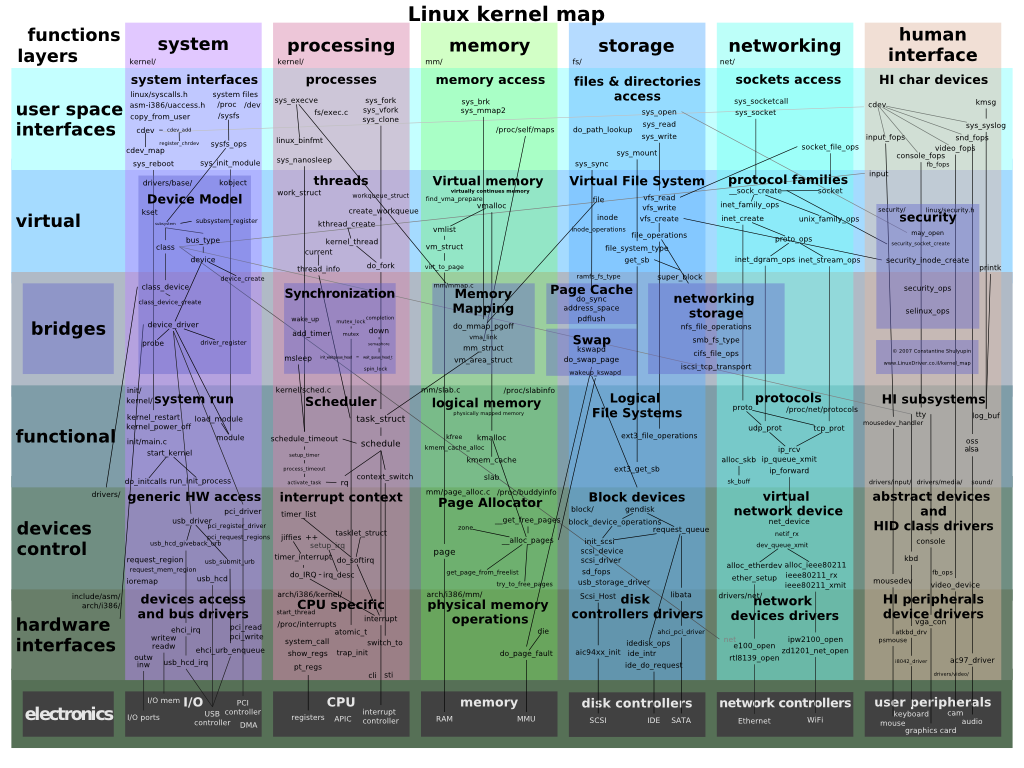
\includegraphics[scale=.40]{articoli/sistema_avanzato/immagini/kernel_map.png}
\caption{mappa del kernel ({\scriptsize fonte: http://it.wikipedia.org/})}
\end{figure*}

La grande complessità di questa mappa ci spaventa ma ci fa rendere conto del lavoro che è stato eseguito per costruire un kernel.\\

Quando è necessario compilare un kernel?

\begin{enumerate}
\item  per far funzionare un componente particolare che non è gestito dal kernel che si utilizza, il cui modulo esiste ma non è stato incluso;
\item per utilizzare l'ultima versione kernel se non è disponibile il pacchetto precompilato;
\item per fare test “particolari” al proprio sistema;
\item a scopi “didattici''.
\end{enumerate}

\hfill {\itshape (fine prima parte)}

\clearpage
\twocolumn[
\begin{center}
\title{\color[cmyk]{1, 0.57, 0, 0.38}{\Huge\bfseries Keyserver e generazione di chiavi GPG \\}} % definisco il titolo dell'articolo
\author{\scriptsize Andrea Veri (averi@fedoraproject.org)} % definisco l'autore e altre informazioni
\date{}
\end{center}
{\color[cmyk]{1, 0.46, 0, 0}\LARGE Vediamo come usare il keyserver Fedora per la generazione di chiavi GPG}\\
\maketitle
\normalsize
\doublespacing
\hfill
]
\onehalfspacing
\lettrine[lines=1, loversize=0.1, lraise=0.1]{\color[cmyk]{0.5, 0, 1, 0}\bfseries D}{}a pochi giorni ha debuttato in Fedora un interessante servizio denominato "Keys" (raggiungibile all'indirizzo http: //keys.fedoraproject.org), si tratta, come si può ben intendere dal nome usato, di un server adibito allo storage di chiavi OpenPGP.\\

Questa tipologia di servizio permette l'inivio e la ricezione di specifiche chiavi di cifratura PGP, le quali vengono selezionate dall'utente a seconda della sua necessità di identificare o di firmare la chiave di un altro soggetto.\\

Ma come funziona esattamente GPG? \\

Il meccanismo risulta essere alquanto semplice ed è, inoltre, similare a quello utilizzato dalla firma digitale, forma di autenticazione dei documenti telematici che oramai sta prendendo piede anche in Italia.\\

GPG, quindi, cifra un determinato messaggio utilizzando una coppia di chiavi (pubblica e privata) generate dall'utente. Il soggetto che riceverà tale messaggio cifrato non dovrà fare altro che verificare l'autenticità della firma e verificarne l'attendibilità. Onde evitare la divulgazione di chiavi false o fittizie e favorire l'associazione chiave pubblica - u\-tente, si è giunti a dare particolare rilevanza al cosiddetto "Web of Trust" (o più comunemente "WoT").\\

Tale concetto è di facile comprensione: si pensi ad un determinato utente che durante un meeting incontra altri individui e dopo aver provveduto ad identificarli tramite un documento d'identità e tramite la verifica della loro impronta digitale (o più comunemente "fingerprint"), firma la loro chiave PGP con la propria, certificandone l'autenticità della provenienza.\\

Questa semplice ma efficace operazione aiuta a rafforzare la rete di fiducia e di conseguenza la stessa credibilità dell'utente stesso.\\

Detto ciò seguirà una brevissima guida che coprirà principalmente tre tematiche:\\
\definecolor{shadecolor}{cmyk}{0, 0, 0, 0.8}
   
\begin{enumerate}
\item la creazione di una chiave PGP 
\item la firma di una chiave PGP altrui
\item la cifratura di un file decifrabile solamente da una determinata chiave
\end{enumerate}

{\bfseries\centering Punto 1. Creazione di una chiave PGP.}\\

\begin{itemize}
\item 1a. Installiamo il software di riferimento.\\
\begin{shaded}
{\color[cmyk]{0, 0, 0, 0}\textdollar\ sudo yum install gnupg}\\
\end{shaded}
\item 1b. Apriamo un terminale e creiamo la nostra chiave di cifratura.\\
\begin{shaded}
{\color[cmyk]{0, 0, 0, 0}\textdollar\ gpg --gen-key}\\
\end{shaded}
Le impostazioni di default, ovvero quelle che otterrete con un semplice 'Invio' ad ogni richiesta di input da parte di GPG, sono solitamente quelle consigliate ad un utente normale.\\
È però consigliabile impostare una data di scadenza alla chiave nel qual caso perdeste o cadesse in mani sbagliate la vostra chiave privata.\\
\item 1c. Appena generata la chiave, inviatela al Keyserver di Fedora, rendondola così pubblicamente disponibile.\\
\begin{shaded}
{\color[cmyk]{0, 0, 0, 0}\textdollar\ gpg --send-keys KEYID --keyserver hkp://keys.fedoraproject.org}\\
\end{shaded}
Per visualizzare il vostro KEYID, vi basterà digitare il seguente comando:
\begin{shaded}
{\color[cmyk]{0, 0, 0, 0}\textdollar\ gpg --list-secret-keys}\\
\end{shaded}
Il KEYID sarà la prima linea numerica che vedrete, ad esempio: sec   4096R/93ECD6F8 2012-01-31\\
\end{itemize}

{\bfseries\centering  Punto 2. Firma di una chiave PGP altrui.}\\

\begin{itemize}
 \item 2a. Otteniamo la chiave che vogliamo firmare dal Keyserver di riferimento.\\
\begin{shaded}
{\color[cmyk]{0, 0, 0, 0}\textdollar\ gpg --recv-key KEYID --keyserver hkp://keys.fedoraproject.org}\\
\end{shaded}
\item 2b. Firmiamo la chiave.\\
\begin{shaded}
{\color[cmyk]{0, 0, 0, 0}\textdollar\ gpg --sign-key KEYID}\\
\end{shaded}
\item 2c. Inviamola nuovamente al keyserver con appresso la nostra firma.\\
\begin{shaded}
{\color[cmyk]{0, 0, 0, 0}\textdollar\ gpg --send-key KEYID}\\
\end{shaded}
\end{itemize}

{\bfseries\centering Punto 3. Cifratura di un file decifrabile solamente da una determinata chiave.}\\

\begin{itemize}
 \item 3a. Otteniamo la chiave di cifratura dell'utente che poi dovrà effettivamente decifrare il nostro messaggio.\\
\begin{shaded}
{\color[cmyk]{0, 0, 0, 0}\textdollar\ gpg --search-keys 'nomeutente@example.com' --keyserver hkp://keys.fedoraproject.org} \\
\end{shaded}
\item 3b. Dopo aver selezionato la chiave corretta dalla lista, verificate che l'importazione è avvenuta correttamente:\\
\begin{shaded}
{\color[cmyk]{0, 0, 0, 0}\textdollar\ gpg --list-keys}
\end{shaded}
\item 3c. Infine, cifrate il messaggio:\\
\begin{shaded}
{\color[cmyk]{0, 0, 0, 0}\textdollar\ gpg --encrypt --recipient 'nomeutente@example.com' nomefile.txt}\\
\end{shaded}
\item 3d. Inviate via mail il file appena generato ('nomefile.txt.gpg') all'utente da voi designato, che potrà, quindi, decifrarlo:\\
\begin{shaded}
{\color[cmyk]{0, 0, 0, 0}\textdollar\ gpg --output nomefile.txt --decrypt nomefile.txt.gpg}
\end{shaded}
In questo caso non servirà importare nessuna chiave dal momento in cui il file di cui sopra è stato cifrato utilizzando la vostra chiave pubblica.\\
\end{itemize}


\clearpage
\twocolumn[
\begin{center}
\title{\color[cmyk]{1, 0.57, 0, 0.38}{\Huge\bfseries Fedora 17\\}} % definisco il titolo dell'articolo
\author{\scriptsize Robert Mayr (robyduck@fedoraonline.it)} % definisco l'autore e altre informazioni
\date{}
\end{center}
{\color[cmyk]{1, 0.46, 0, 0}\LARGE Fedora 17 - una panoramica sulle novità}\\
\maketitle
\normalsize
\doublespacing
\hfill
]
\onehalfspacing
\lettrine[lines=1, loversize=0.1, lraise=0.1]{\color[cmyk]{0.5, 0, 1, 0}\bfseries E'}{} notizia di pochi giorni fa l'annuncio di {\itshape Dennis Gilmore} riguardante l'uscita della versione {\itshape alpha} di Fedora 17 ``Beefy Miracle'', per la quale sono previste le caratteristiche che possiamo vedere complete a questo indirizzo: {\itshape http://fedo\\raproject.org/wiki/Releases/17/Feature\\List\#Fedora\_17\_Accepted\_Features}.\\

La roadmap per il rilascio della versione {\itshape stable} si può trovare alla pagina {\itshape http://\\fedoraproject.org/wiki/Schedule}.\\

\begin{figure}[htbp]
\centering
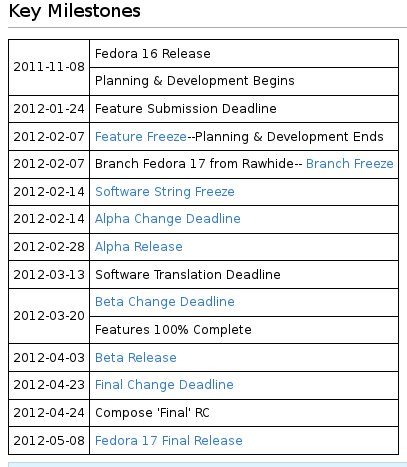
\includegraphics[scale=.60]{articoli/notizie/immagini/roadmap_wiki.jpeg}
\caption{roadmap per Fedora 17 {\itshape Beefy Miracle}}
\end{figure}


Come al solito la lista delle features accettate è molto differenziata, ma tra queste possiamo rilevarne alcune molto importanti sia per gli utenti finali che per chi è interessato al sistema ed allo sviluppo:
\begin{itemize}
\item Gnome 3.4.
\item KDE 4.8.
\item Gimp 2.8.
\item Kernel 3.3.
\item GCC 4.7.x.
\item PHP 5.4.
\item Software rendering for gnome-shell.
\item Move all to /usr.
\item ABRT Backtrace Deduplication Service.
\item Eucalyptus.
\item Firewalld.
\item KVM Live Block Migration.
\item NetworkManager Hotspots.
\item Riak.
\end{itemize}

Vediamone alcune più dettagliatamente:\\

\begin{center}
{\centering\bfseries Gnome 3.4}
\end{center}
Tra le novità spicca, anche se ancora in fase di sviluppo e con qualche ostacolo di trademark, {\itshape Boxes} che sempificherà l'accesso ad altri sistemi operativi, siano essi fisici, virtuali o raggiungibili via rete. Sarà incluso anche l'accesso remoto, il tutto utilizzando la tecnologia Qemu. Nonostante lo sviluppo di virt-manager {\itshape Boxes} si pone l'obiettivo di mettere a disposizione dell'utente un'interfaccia più amichevole.

\begin{figure}[!h]
\centering
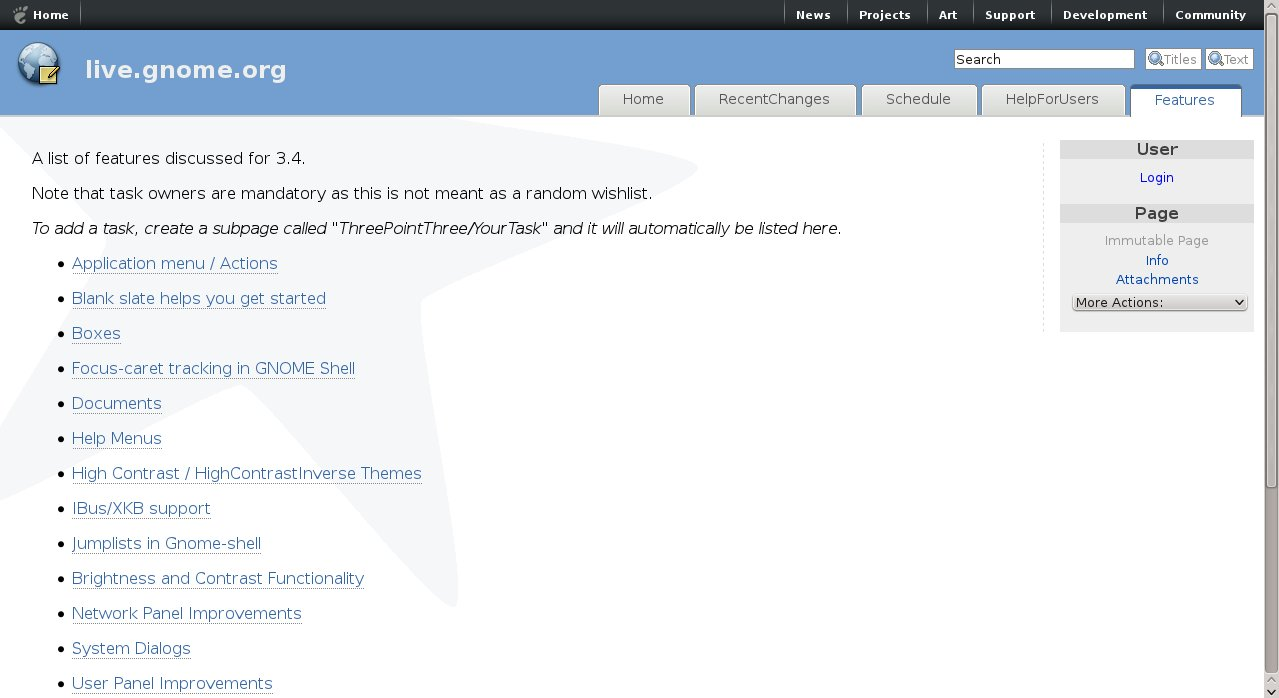
\includegraphics[scale=.20]{articoli/notizie/immagini/gnome_3_4.jpeg}
\caption{live.gnome.org}
\end{figure}
\begin{center}
{\centering\bfseries KDE 4.8}
\end{center}
In questa versione, l'utility{\itshape KDE Power Management System Settings} è stata aggiornata sia per quanto riguarda l'interfaccia utente che per il layout. Sono stati introdotti miglioramenti per {\itshape Dolphin}, {\itshape Gwenview}, {\itshape KMail} (non si dovrebbero riscontrare i problemi di sicurezza e stabilità delle versioni precedenti), {\itshape Kate} e molto altro.

\begin{figure}[htbp]
\centering
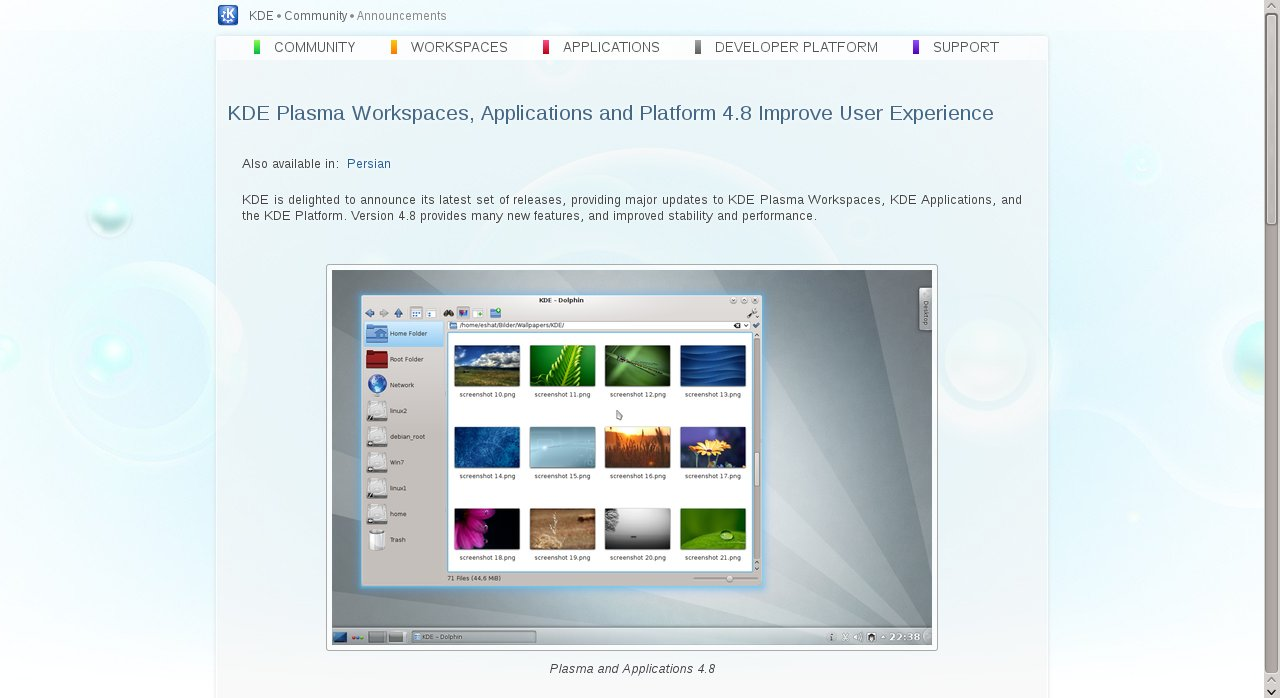
\includegraphics[scale=.20]{articoli/notizie/immagini/kde_4_8.jpeg}
\caption{kde.org}
\end{figure}

\begin{center}
{\centering\bfseries Kernel 3.3}
\end{center}
Uno dei cambiamenti nella versione 3.3 del kernel è dovuto all'inserimento di un nuovo meccanismo per regolare la dimensione dei filesystems ext4; questo meccanismo dovrebbe ora lavorare più velocemente. Miglioramenti sono stati apportati anche per l'audio HDMI su tipologie di chipset AMD e Nvidia. Sono stati raggruppati, inoltre, alcuni dispositivi ethernet in un unico dispositivo virtuale. E' stato inserito il supporto a Open vSwitch. Il filesystem btrfs è stato ottimizzato per operazioni con volumi RAID ed è inserita in via sperimentale la verifica dell'integrità dei dischi in alcune operazioni.

\begin{figure}[htbp]
\centering
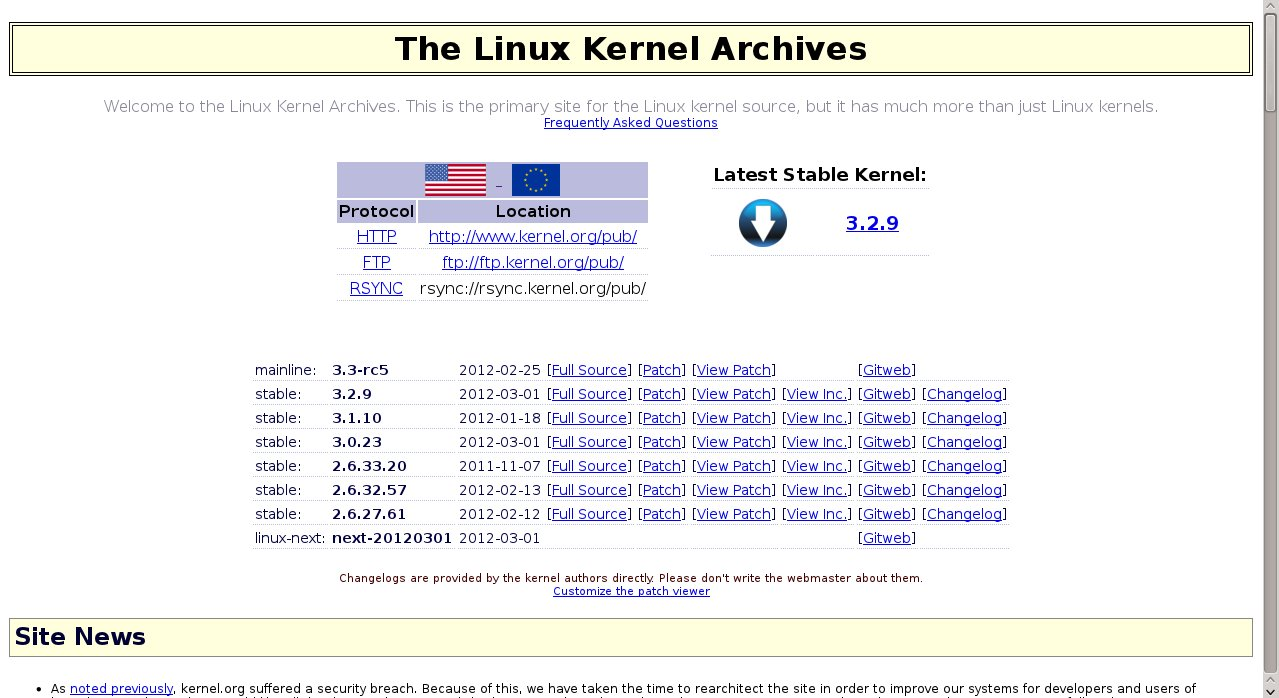
\includegraphics[scale=.20]{articoli/notizie/immagini/kernel.jpeg}
\caption{kernel.org}
\end{figure}

\begin{center}
{\centering\bfseries Software rendering for gnome-shell}
\end{center}
Gnome-shell sarà in grado di funzionare anche con gran parte di quelle schede grafiche che non supportano l'accelerazione 3D, un enorme passo avanti per quanto riguarda l'usabilità del DE di default.

\begin{center}
{\centering\bfseries Move all to /usr}
\end{center}
Come già visto nell'articolo relativo ai pacchetti rpm, è stato stabilito lo spostamento di tutte le /lib e /bin sotto la directory /usr. Di fatto, le directory /lib, /lib64, /bin e /sbin conterranno soltanto dei link simbolici ai file che si troveranno sotto la directory /usr.

\begin{center}
{\centering\bfseries ABRT Backtrace Deduplication Service}
\end{center}
Durante l'inserimento di un nuovo bug nel RedHat Bugzilla, ABRT controllerà se ne è già stato aperto uno per lo stesso problema, onde evitare duplicati.

\begin{center}
{\centering\bfseries Eucalyptus}
\end{center}
Eucalyptus è un software cloud computing per l'utilizzo privato, che permette di utilizzare le infrastrutture esistenti per creare clouds per computer, memoria di massa e rete. Nelle novità del cloud computing si inserisce anche il toolkit OpenNebula.

\begin{center}
{\centering\bfseries Firewalld - default firewall solution}
\end{center}
Il nuovo firewall di default sostituisce i servizi iptables, iptables-ipv6 e ebtables.

\begin{center}
{\centering\bfseries KVM Live Block Migration}
\end{center}
KVM avrà la possibilità di migrare immagini del disco, mentre questo è in "funzione" (live block migration). oVirt è ancora in fase sperimentale, ma dovrebbe essere in grado di virtualizzare server, fare migrazioni live block e molto altro.

\begin{center}
{\centering\bfseries NetworkManager Hotspots}
\end{center}
Questa aggiunta mette NetworkManager nelle condizioni di funzionare come Access Point.

\begin{center}
{\centering\bfseries Riak}
\end{center}
Il database in clustering NoSQL viene incluso nei repo di Fedora. Riak avrà anche una consolle di amministrazione dei cluster, che rende più agevole la loro gestione.\\

Per concludere, un'ultima notizia: il filesystem di default rimarrà ext4 (il quale avrà il supporto per gestire dischi oltre i 16TB) in quanto btrfs è slittato, per alcune incompatibilità e restrizioni di anaconda, almeno alla versione 18.\\

Il resto lo scopriremo all'uscita di {\bfseries Fedora 17 ``Beefy Miracle''} l' 8 Maggio 2012, salvo ritardi.\\

\clearpage
\ThisTileWallPaper{21cm}{29,7cm}{articoli/varie/immagini/ultima_copertina.png}
\onecolumn
\thispagestyle{empty}
\vspace*{6,5cm}
\color[cmyk]{0, 0, 0, 0}
\centering
\textsc{\LARGE FOLIO - Il webmagazine di FedoraOnLine (http://www.fedoraonline.it)}\\[1.0cm]
\textsc{\Large rivista non professionale tematica e libera creata dai lettori di FedoraOnLine, scaricabile e dai contenuti forniti dagli utenti Fedora in italia e nel mondo.}\\[0.5cm]
\begin{figure}[htbp]
\centering

\includegraphics[scale=1.0]{immagini/logo/cc.png}
\end{figure}
{\bfseries Folio ed i suoi contenuti sono distribuiti con licenza creative commons, reperibile a questo link: http://creativecommons.org/licenses/by-sa/3.0/it/ }\\[0.4cm]
{\doublespacing}
\begin{tiny}
\begin{spacing}{1.0}
Questa rivista segue le linee guida dettate dal Fedora Project reperibile all'indirizzo  http://fedoraproject.org/wiki/Legal:Trademark\_guidelines:\\
{\bfseries Publications}\\
``It is permissible to use the Fedora trademarks in the title and content of a publication, provided that:
    the use is clearly in reference to the Fedora Project or its software
    the use does not imply sponsorship or endorsement by Red Hat or the Fedora Project
    Proper trademark symbols are used in connection with the Fedora Trademarks and the trademark attribution statement must appear as explained in Proper Trademark Use.'' \\
Fedora\textregistered and the Infinity design logo are trademarks of Red Hat, Inc.
\end{spacing}
\end{tiny}
\rule{\textwidth}{0.5mm}\\
\vfill
\noindent


\end{document}
